\documentclass[10pt,a4paper]{article}

\usepackage[T1]{fontenc}
\usepackage[utf8]{inputenc}
\usepackage[a4paper,margin=15mm,top=14mm,bottom=16mm]{geometry}
\usepackage{graphicx}
\usepackage{booktabs}
\usepackage{array}
\usepackage{caption}
\usepackage{xcolor}
\usepackage{microtype}
\microtypesetup{expansion=false}
\usepackage[hidelinks]{hyperref}
\emergencystretch=2em

\graphicspath{{../}}
% Generated by report/generate_values.py; do not edit metrics by hand.
\newcommand{\TaskZeroAccuracy}{92.20}
\newcommand{\TaskZeroLoss}{0.1899}
\newcommand{\TaskZeroCorrect}{260}
\newcommand{\TaskZeroTestSize}{282}
\newcommand{\TaskZeroValAccuracy}{90.39}
\newcommand{\TaskZeroBestEpoch}{13}
\newcommand{\TaskZeroEpochsRun}{19}
\newcommand{\TaskZeroTrainingSeconds}{112.89}
\newcommand{\TaskZeroCMZeroZero}{134}
\newcommand{\TaskZeroCMZeroOne}{8}
\newcommand{\TaskZeroCMOneZero}{14}
\newcommand{\TaskZeroCMOneOne}{126}
\newcommand{\TaskOneTrials}{53}
\newcommand{\TaskOneComplete}{20}
\newcommand{\TaskOnePruned}{33}
\newcommand{\TaskOneTrialEpochs}{5}
\newcommand{\TaskOneBestTrial}{42}
\newcommand{\TaskOneValAccuracy}{96.44}
\newcommand{\TaskOneTestAccuracy}{95.39}
\newcommand{\TaskOneTestLoss}{0.1473}
\newcommand{\TaskOneCorrect}{269}
\newcommand{\TaskOneTestSize}{282}
\newcommand{\TaskOneGain}{3.19}
\newcommand{\TaskOneBestEpoch}{5}
\newcommand{\TaskOneTrainingSeconds}{47.40}
\newcommand{\TaskOneLearningRate}{0.011812}
\newcommand{\TaskOneBatchSize}{32}
\newcommand{\TaskOneOptimizer}{AdamW}
\newcommand{\TaskOneWeightDecay}{9.39e-07}
\newcommand{\TaskOneDepth}{3}
\newcommand{\TaskOneChannels}{16}
\newcommand{\TaskOneDropout}{0.2}
\newcommand{\TaskOneLRImportance}{41.68}
\newcommand{\TaskOneBatchImportance}{37.45}
\newcommand{\TaskTwoFirstFailure}{0.10}
\newcommand{\TaskTwoCleanAccuracy}{92.20}
\newcommand{\TaskTwoRealizations}{5}
\newcommand{\TaskTwoFailureDrop}{20.00}
\newcommand{\TaskTwoChanceThreshold}{60.00}
\newcommand{\TaskThreeCorrectZeroIndex}{1}
\newcommand{\TaskThreeCorrectOneIndex}{0}
\newcommand{\TaskThreeFalsePositiveIndex}{88}
\newcommand{\TaskThreeFalseNegativeIndex}{7}
\newcommand{\TaskThreeFalsePositiveConfidence}{97.86}
\newcommand{\TaskThreeFalseNegativeConfidence}{61.94}
\newcommand{\TaskFourAccuracy}{92.20}
\newcommand{\TaskFourFalsePositives}{8}
\newcommand{\TaskFourFalseNegatives}{14}
\newcommand{\TaskFourMacroFOne}{92.19}
\newcommand{\TaskFourClassZeroPrecision}{90.54}
\newcommand{\TaskFourClassZeroRecall}{94.37}
\newcommand{\TaskFourClassZeroFOne}{92.41}
\newcommand{\TaskFourClassZeroSupport}{142}
\newcommand{\TaskFourClassOnePrecision}{94.03}
\newcommand{\TaskFourClassOneRecall}{90.00}
\newcommand{\TaskFourClassOneFOne}{91.97}
\newcommand{\TaskFourClassOneSupport}{140}
\newcommand{\TaskFiveNTNT}{92.20}
\newcommand{\TaskFiveNTUT}{82.49}
\newcommand{\TaskFiveUTNT}{92.55}
\newcommand{\TaskFiveUTUT}{93.79}
\newcommand{\TaskFiveNTUTLoss}{0.3124}
\newcommand{\TaskFiveUTNTLoss}{0.2431}
\newcommand{\TaskFiveNTUTSourceDrop}{9.71}
\newcommand{\TaskFiveNTUTTargetGap}{11.30}
\newcommand{\TaskFiveNTBestEpoch}{13}
\newcommand{\TaskFiveUTBestEpoch}{29}
\newcommand{\TaskFiveNTTrainingSeconds}{83.64}
\newcommand{\TaskFiveUTTrainingSeconds}{87.11}
\newcommand{\TaskFiveNTUTClassZeroErrors}{16}
\newcommand{\TaskFiveNTUTClassOneErrors}{15}
\newcommand{\TaskTwoRows}{%
0.00 & 92.20 & 0.00 & 0.00 & No \\
0.05 & 79.01 & 0.30 & 13.19 & No \\
0.10 & 50.78 & 0.16 & 41.42 & \textbf{Yes} \\
0.15 & 50.35 & 0.00 & 41.84 & \textbf{Yes} \\
0.20 & 50.35 & 0.00 & 41.84 & \textbf{Yes} \\
0.30 & 50.35 & 0.00 & 41.84 & \textbf{Yes} \\
0.50 & 50.35 & 0.00 & 41.84 & \textbf{Yes} \\
}
\newcommand{\TaskThreeRows}{%
1 & Correct class 0 & 0 & 0 & 97.86 \\
0 & Correct class 1 & 1 & 1 & 64.62 \\
88 & False positive & 0 & 1 & 97.86 \\
7 & False negative & 1 & 0 & 61.94 \\
}


\definecolor{accent}{RGB}{27,83,125}
\hypersetup{colorlinks=true,linkcolor=accent,citecolor=accent,urlcolor=accent}
\captionsetup{font=small,labelfont=bf,skip=3pt}
\setlength{\parindent}{0pt}
\setlength{\parskip}{3pt}
\setlength{\textfloatsep}{6pt}
\setlength{\floatsep}{6pt}
\setlength{\intextsep}{6pt}
\renewcommand{\arraystretch}{1.08}
\raggedbottom

\newcommand{\TaskPage}[2]{%
  \clearpage
  \section{Task #1: #2}\label{task:#1:start}%
}
\newcommand{\TaskEnd}[1]{\label{task:#1:end}}
\newcommand{\RunHead}[1]{\par\smallskip\noindent\textbf{#1.}\ }
\newcommand{\CodePath}[1]{%
  \par\smallskip\noindent\textbf{Code location: }\nolinkurl{#1}.%
}

\begin{document}

\begin{center}
  {\LARGE\bfseries CNN Classification Study\par}
  \vspace{2mm}
  {\large Yagiz Koc\par}
  \vspace{1mm}
  {\large June 26, 2026\par}
\end{center}

\section*{Introduction}

This report covers the completed tasks \textbf{0, 1, 2, 3, 4, and 5}. Tasks 0--4 use
NT as the graded dataset. Task 5 additionally uses the valid-label UT dataset for the prescribed NT$\rightarrow$UT and UT$\rightarrow$NT experiments; ASB is never used for graded training or evaluation.

All displayed values are generated from the saved JSON/CSV artifacts by
\nolinkurl{report/generate_values.py}. The generator checks figure existence, hashes its
inputs, and verifies that the repeated Task 0 result agrees across Tasks 2, 4, and 5.
Train, validation, and test roles remain separated: model fitting uses train, selection uses
validation, and test is accessed only after checkpoint and preprocessing lock.

\vspace{1cm}

\begin{table}[h]
\centering
\small
\caption{Completed tasks and explicit report page ranges.}
\label{tab:task-pages}
\begin{tabular}{clc}
\toprule
Task & Deliverable & Pages \\
\midrule
0 & Baseline CNN & \pageref{task:0:start}--\pageref{task:0:end} \\
1 & Optuna hyperparameter study & \pageref{task:1:start}--\pageref{task:1:end} \\
2 & Gaussian-noise robustness & \pageref{task:2:start}--\pageref{task:2:end} \\
3 & Activation maps and Grad-CAM & \pageref{task:3:start}--\pageref{task:3:end} \\
4 & Confusion-matrix error analysis & \pageref{task:4:start}--\pageref{task:4:end} \\
5 & NT/UT cross-dataset generalization & \pageref{task:5:start}--\pageref{task:5:end} \\
\bottomrule
\end{tabular}
\end{table}

\TaskPage{0}{Baseline CNN}

\RunHead{Approach}
The CNN uses three $3\times3$ convolution/ReLU stages with
16, 32, and 64 channels, two max-pooling operations, global average pooling, and a
two-logit head. Raw $128\times128$ float32 images in $[0,1]$ are used without augmentation
or normalization. Adam with learning rate $10^{-3}$ and batch size 64
updates NT/train; minimum NT/val cross-entropy selects the checkpoint, with patience 6.
\\
Concretely, the baseline has 23,426 trainable parameters
with the exact stack:
input \(1\times128\times128\) \(\rightarrow\) Conv(1,16) \(\rightarrow\) ReLU
\(\rightarrow\) Pool \(\rightarrow\) Conv(16,32) \(\rightarrow\) ReLU \(\rightarrow\) Pool
\(\rightarrow\) Conv(32,64) \(\rightarrow\) ReLU \(\rightarrow\) AvgPool
\(\rightarrow\) Linear(64,2).
Loss is accumulated sample-wise, so partial final batches are weighted correctly. 
\\
The model is not imported from a pretrained source: \texttt{model.py} defines the architecture,
\texttt{train.py} instantiates it from a fixed seed, builds separate NT/train and NT/val loaders,
optimizes cross-entropy on NT/train, evaluates after each epoch on NT/val, and records the full
history. Only after the validation-selected checkpoint and preprocessing metadata are saved does
the script reload \texttt{best\_model.pt} and open NT/test for the final metric.

\RunHead{Running the code and predicting new samples}
From the repository root, the saved run can be reproduced with the documented launcher:
\begin{small}
	\begin{verbatim}
		conda run -n cnn_project python tasks/task_0_baseline_cnn/train.py \
		--seed 42 --epochs 30 --batch-size 64 --learning-rate 0.001 \
		--device cpu --workers 0 --output-dir tasks/task_0_baseline_cnn/results
	\end{verbatim}
\end{small}
This command writes the checkpoint, configuration, history, metrics, and training plot in
\nolinkurl{tasks/task_0_baseline_cnn/results/}. For a quick prediction test on an existing NT
sample, export a PNG from the supplied NPZ file and then pass that image to the dedicated
prediction script:
\begin{small}
	\begin{verbatim}
		conda run -n cnn_project python tasks/task_0_baseline_cnn/import_nt_images.py \
		--split test --output-dir tasks/task_0_baseline_cnn/imported_images 0
		conda run -n cnn_project python tasks/task_0_baseline_cnn/predict.py \
		tasks/task_0_baseline_cnn/imported_images/nt_test_0000_label1.png --device cpu
	\end{verbatim}
\end{small}
\texttt{predict.py} also accepts a new external image path, converts it to grayscale, resizes it
to $128\times128$, scales pixels to $[0,1]$, loads \texttt{best\_model.pt}, verifies the locked
preprocessing metadata, and prints the predicted label plus both class probabilities.

\RunHead{Results}
Training stopped after \TaskZeroEpochsRun{} epochs and restored epoch
\TaskZeroBestEpoch{}. Table~\ref{tab:t0-results} and Figure~\ref{fig:t0-curves} report the
locked result.

\begin{center}
\begin{minipage}[t]{0.4\linewidth}
\centering
\captionof{table}{Task 0 validation and NT/test results.}
\label{tab:t0-results}
\small
\begin{tabular}{lr}
\toprule
Metric & Value \\
\midrule
Best validation accuracy & \TaskZeroValAccuracy\% \\
Test accuracy & \TaskZeroAccuracy\% \\
Correct / test samples & \TaskZeroCorrect/\TaskZeroTestSize \\
Test cross-entropy & \TaskZeroLoss \\
Training time (CPU) & \TaskZeroTrainingSeconds{} s \\
Confusion matrix & \texttt{[[\TaskZeroCMZeroZero,\TaskZeroCMZeroOne],[\TaskZeroCMOneZero,\TaskZeroCMOneOne]]} \\
\bottomrule
\end{tabular}
\end{minipage}
\begin{minipage}[t]{0.7\linewidth}
\centering
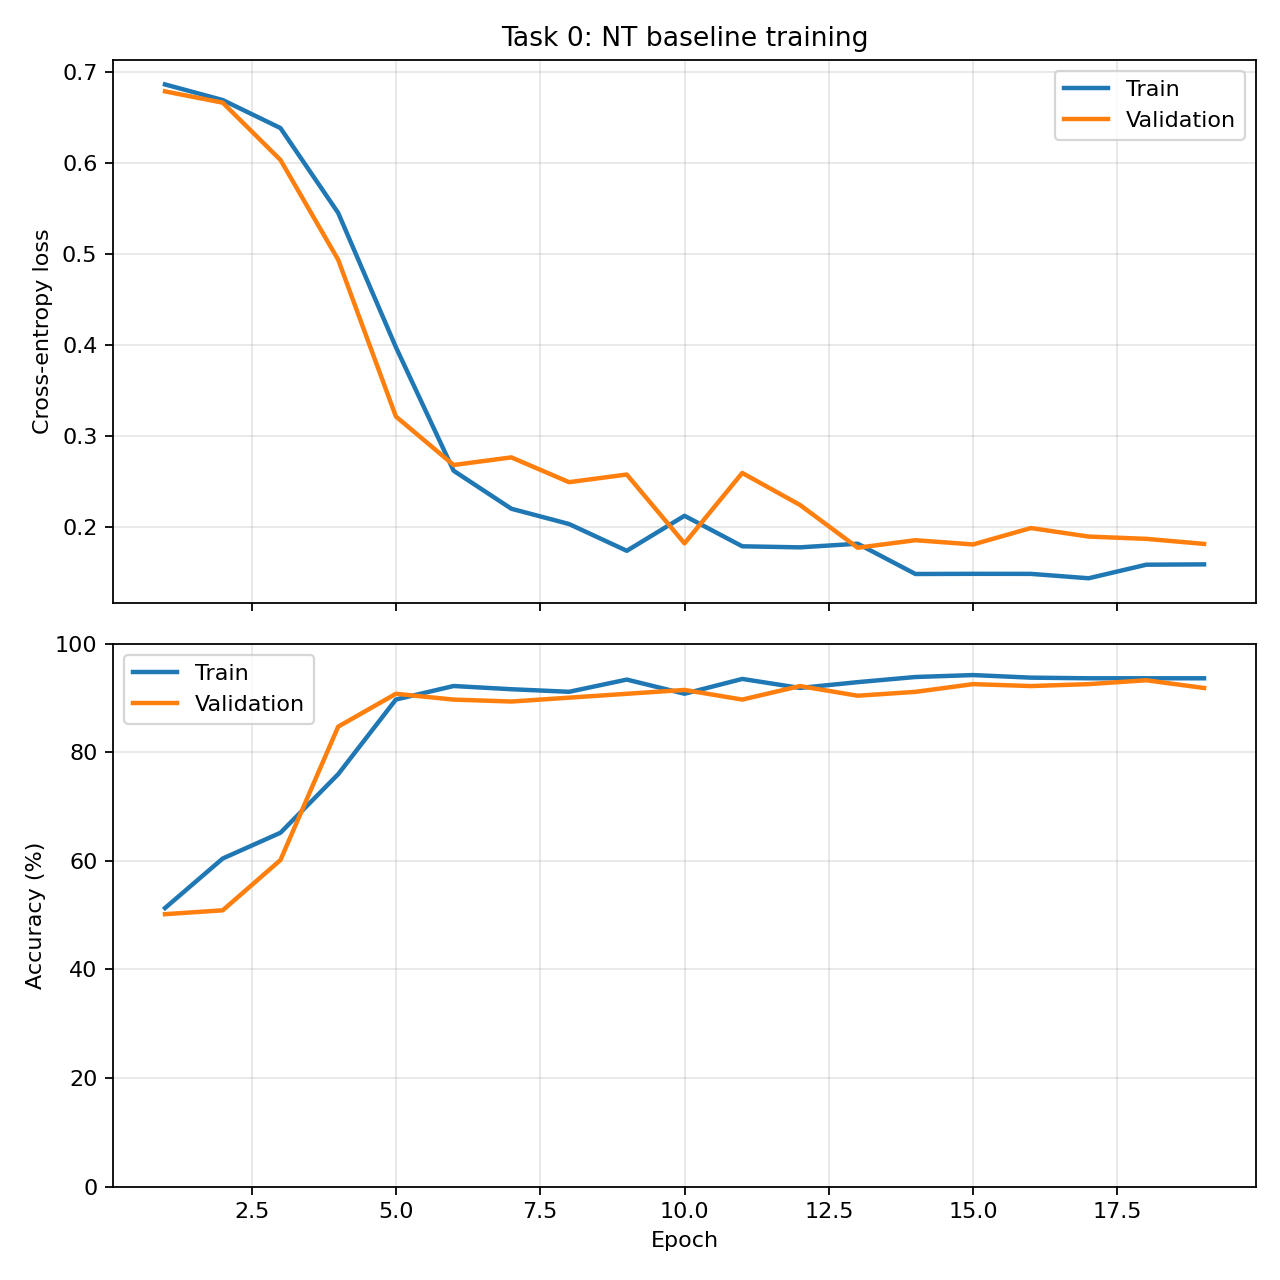
\includegraphics[width=0.7\linewidth]{tasks/task_0_baseline_cnn/results/training_curves.png}
\captionof{figure}{Sample-weighted train/validation loss and accuracy.}
\label{fig:t0-curves}
\end{minipage}
\end{center}

\RunHead{Discussion}
Learning is rapid through approximately epoch 6, after which validation
loss oscillates around a plateau; final accuracy is \TaskZeroAccuracy\%. The compact convolutional hierarchy is sufficient to learn useful
NT texture/edge features, consistent with the local-bias advantages of CNNs. However, this is one seed, one NT split, and no augmentation;
the test result does not establish robustness or cross-domain performance.

\CodePath{tasks/task_0_baseline_cnn/}
\TaskEnd{0}

\TaskPage{1}{Optuna Hyperparameter Study}

\RunHead{Approach}
A seeded Optuna TPE study with median pruning searches learning rate,
batch size, optimizer, weight decay, depth, channel width, and dropout. Each trial uses
NT/train and NT/val for \TaskOneTrialEpochs{} epochs; NT/test remains unopened. The study
contains \TaskOneTrials{} trials (\TaskOneComplete{} complete, \TaskOnePruned{} pruned).
The selected configuration is retrained from scratch and locked by validation performance.
The objective function maximizes the best NT/val accuracy achieved within a short trial:
Optuna samples one hyperparameter configuration, the script builds the corresponding
\texttt{SimpleCNN}, trains it only on NT/train, evaluates NT/val after each epoch, reports
the best validation accuracy to Optuna, and allows the median pruner to stop weak trials.
This produced the exploratory trial table and the optimization-history/importance plots.
After the search, trial \TaskOneBestTrial{} was not used directly as a final model; its
configuration was retrained from scratch with the same fixed NT splits, selected again on
validation performance, saved as \texttt{final\_model.pt}, reloaded, and only then evaluated
once on NT/test.

\RunHead{Running the code and predicting new samples}
The full search and locked final evaluation are reproduced from the repository root with:
\begin{small}
	\begin{verbatim}
		conda run -n cnn_project python tasks/task_1_hyperparameter/optuna_search.py \
		--trials 24 --trial-epochs 5 --min-completed-trials 20 \
		--final-epochs 30 --final-patience 6 --seed 42 --device cpu --workers 0 \
		--output-dir tasks/task_1_hyperparameter/results \
		--study-name task1_nt_optuna --reset-study
	\end{verbatim}
\end{small}
The command writes the Optuna database, flattened trials CSV, selected parameters, final
checkpoint, final metrics, and search plots. Because pruning can stop many trials early, the
script continues until the requested number of completed trials is reached. For prediction with
the optimal saved model, first export a sample PNG from NT and then call the Task 1 predictor:
\begin{small}
	\begin{verbatim}
		conda run -n cnn_project python tasks/task_1_hyperparameter/import_nt_images.py \
		1 --split test
		conda run -n cnn_project python tasks/task_1_hyperparameter/predict.py \
		tasks/task_1_hyperparameter/imported_images/nt_test_0001_label0.png --device cpu
	\end{verbatim}
\end{small}
\texttt{predict.py} defaults to \texttt{tasks/task\_1\_hyperparameter/results/final\_model.pt}.
It also accepts a repository-relative or absolute external image path, applies the same
grayscale resize and $[0,1]$ scaling used by Task 0, verifies the checkpoint preprocessing
metadata, and prints the predicted class plus both softmax scores.

\RunHead{Results}
\begin{table}[h]
\centering
\small
\caption{Optuna-selected configuration and locked performance.}
\label{tab:t1-results}
\begin{tabular}{llllll}
\toprule
Trial & Optimizer & LR & Batch & Depth/base width & Dropout \\
\midrule
\TaskOneBestTrial & \TaskOneOptimizer & \TaskOneLearningRate & \TaskOneBatchSize &
\TaskOneDepth/\TaskOneChannels & \TaskOneDropout \\
\midrule
\multicolumn{2}{l}{Best validation accuracy} & \multicolumn{1}{l}{\TaskOneValAccuracy\%} &
\multicolumn{2}{l}{Final NT/test accuracy} & \TaskOneTestAccuracy\% \\
\multicolumn{2}{l}{Weight decay} & \multicolumn{1}{l}{\TaskOneWeightDecay} &
\multicolumn{2}{l}{Correct / test samples} & \TaskOneCorrect/\TaskOneTestSize \\
\bottomrule
\end{tabular}
\end{table}

\begin{figure}[h]
\centering
\begin{minipage}{0.49\linewidth}
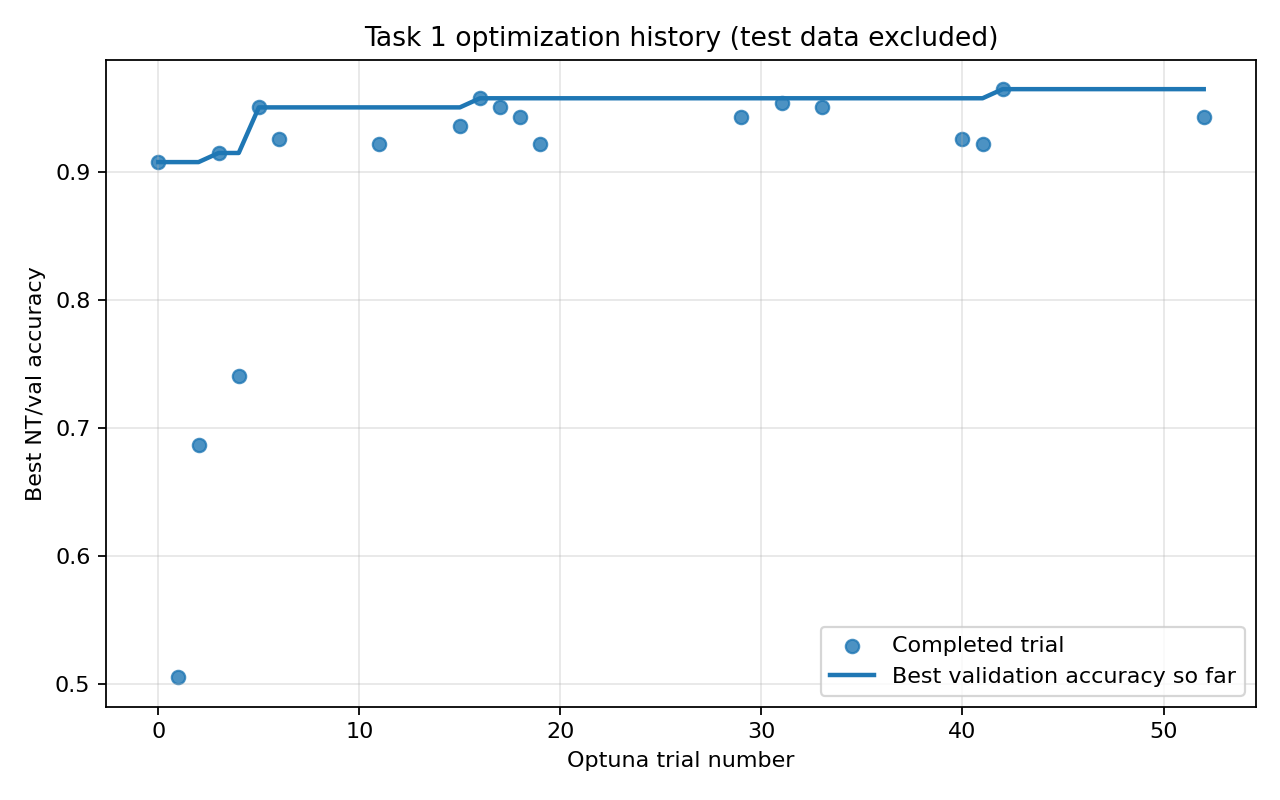
\includegraphics[width=\linewidth]{tasks/task_1_hyperparameter/results/optimization_history.png}
\end{minipage}\hfill
\begin{minipage}{0.49\linewidth}
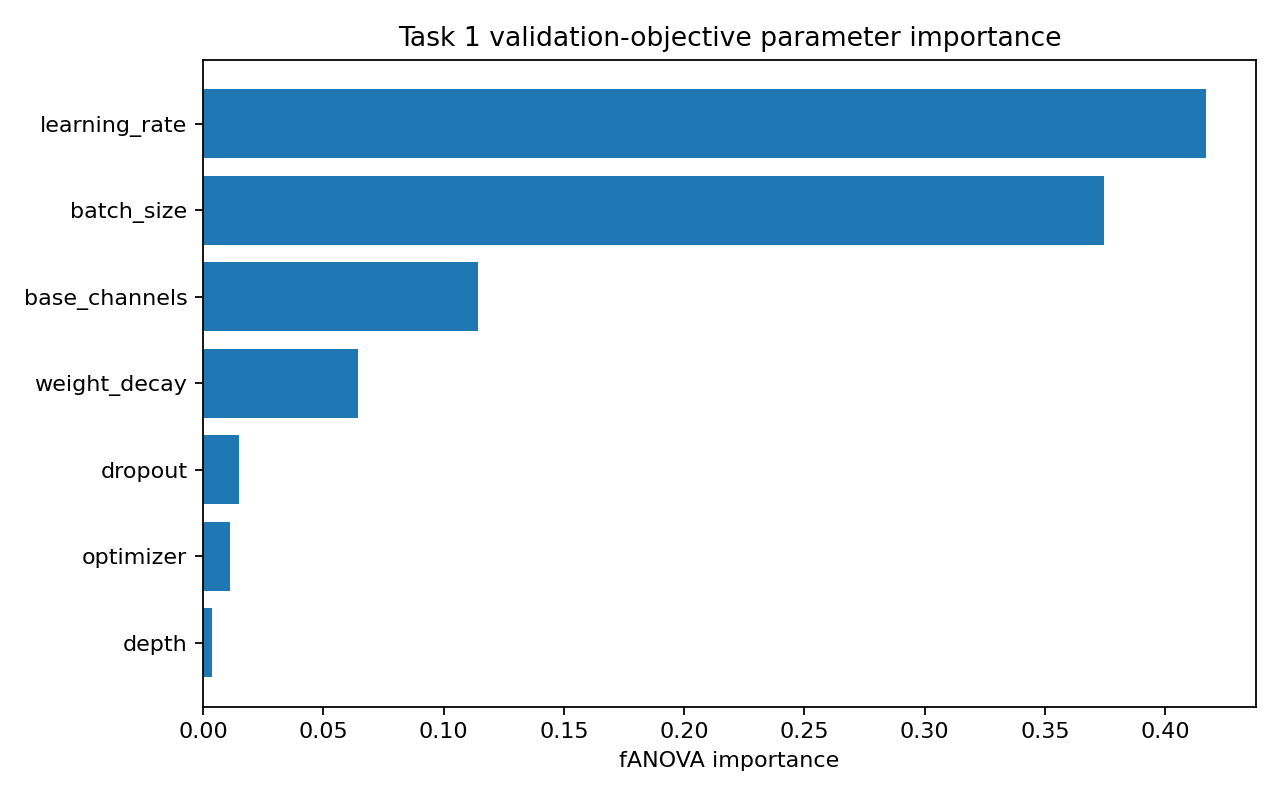
\includegraphics[width=\linewidth]{tasks/task_1_hyperparameter/results/parameter_importance.png}
\end{minipage}
\caption{Validation-only optimization history (left) and inspected fANOVA importance (right).}
\label{fig:t1-search}
\end{figure}

\RunHead{Discussion}
The selected model reaches \TaskOneTestAccuracy\%, a
\TaskOneGain-point gain over Task 0. Learning rate and batch size contribute
\TaskOneLRImportance\% and \TaskOneBatchImportance\% of the local importance estimate.
The optimization primarily improved the training dynamics, while AdamW,
dropout, and the retained three-stage width provided the best sampled combination.

\CodePath{tasks/task_1_hyperparameter/}
\TaskEnd{1}

\TaskPage{2}{Robustness to Gaussian Noise}

\RunHead{Approach}
The frozen Task 0 checkpoint is evaluated at
$\sigma\in\{0,.05,.10,.15,.20,.30,.50\}$. Gaussian noise is added in the original
$[0,1]$ image domain and clamped before applying checkpoint preprocessing. Each nonzero
$\sigma$ uses \TaskTwoRealizations{} deterministic realizations. Failure means accuracy
$\leq\TaskTwoChanceThreshold\%$ or a drop $\geq\TaskTwoFailureDrop$ percentage points,
following the corruption-testing motivation of Hendrycks and Dietterich (2019).

The script reloads the locked Task 0 checkpoint and its preprocessing metadata, evaluates
NT/test at each $\sigma$, writes raw per-realization CSV rows and summary JSON/CSV files,
and saves the accuracy curve and fixed-sample gallery shown below.

\RunHead{Running the code}
The full workflow of this task is reproduced from the repository root with:
\begin{small}
	\begin{verbatim}
		conda run -n cnn_project python tasks/task_2_robustness/noise_analysis.py \
		--checkpoint tasks/task_0_baseline_cnn/results/best_model.pt \
		--realizations 5 --noise-seed 2026 --batch-size 64 --device cpu --workers 0 \
		--output-dir tasks/task_2_robustness/results
	\end{verbatim}
\end{small}

\RunHead{Results}
\begin{center}
\begin{minipage}[t]{0.43\linewidth}
\centering
\captionof{table}{NT/test accuracy under noise; SD and drop are percentage points.}
\label{tab:t2-noise}
\scriptsize
\begin{tabular}{rrrrc}
\toprule
$\sigma$ & Mean (\%) & SD & Drop & Failed \\
\midrule
\TaskTwoRows
\bottomrule
\end{tabular}
\end{minipage}

\begin{minipage}[t]{0.54\linewidth}
\centering
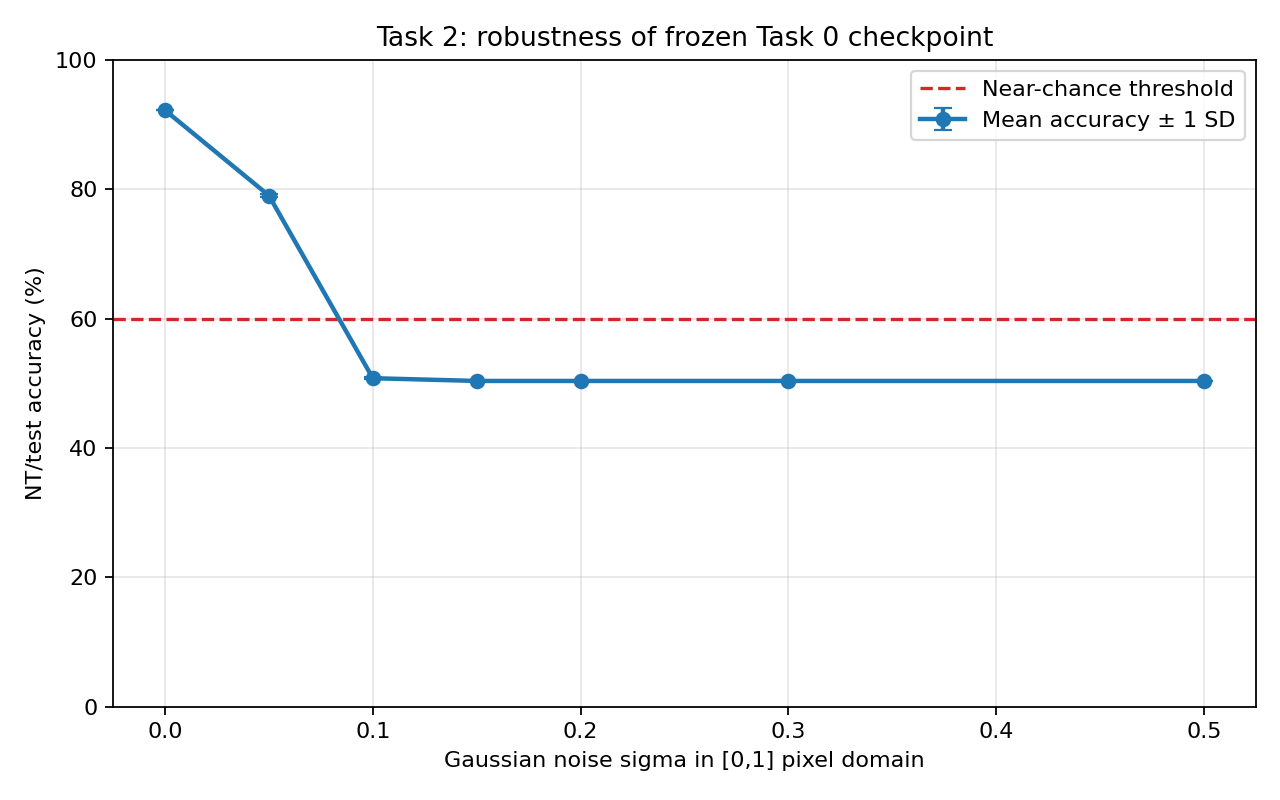
\includegraphics[width=\linewidth]{tasks/task_2_robustness/results/accuracy_vs_sigma.png}
\captionof{figure}{Mean accuracy with one-SD uncertainty.}
\label{fig:t2-curve}
\end{minipage}

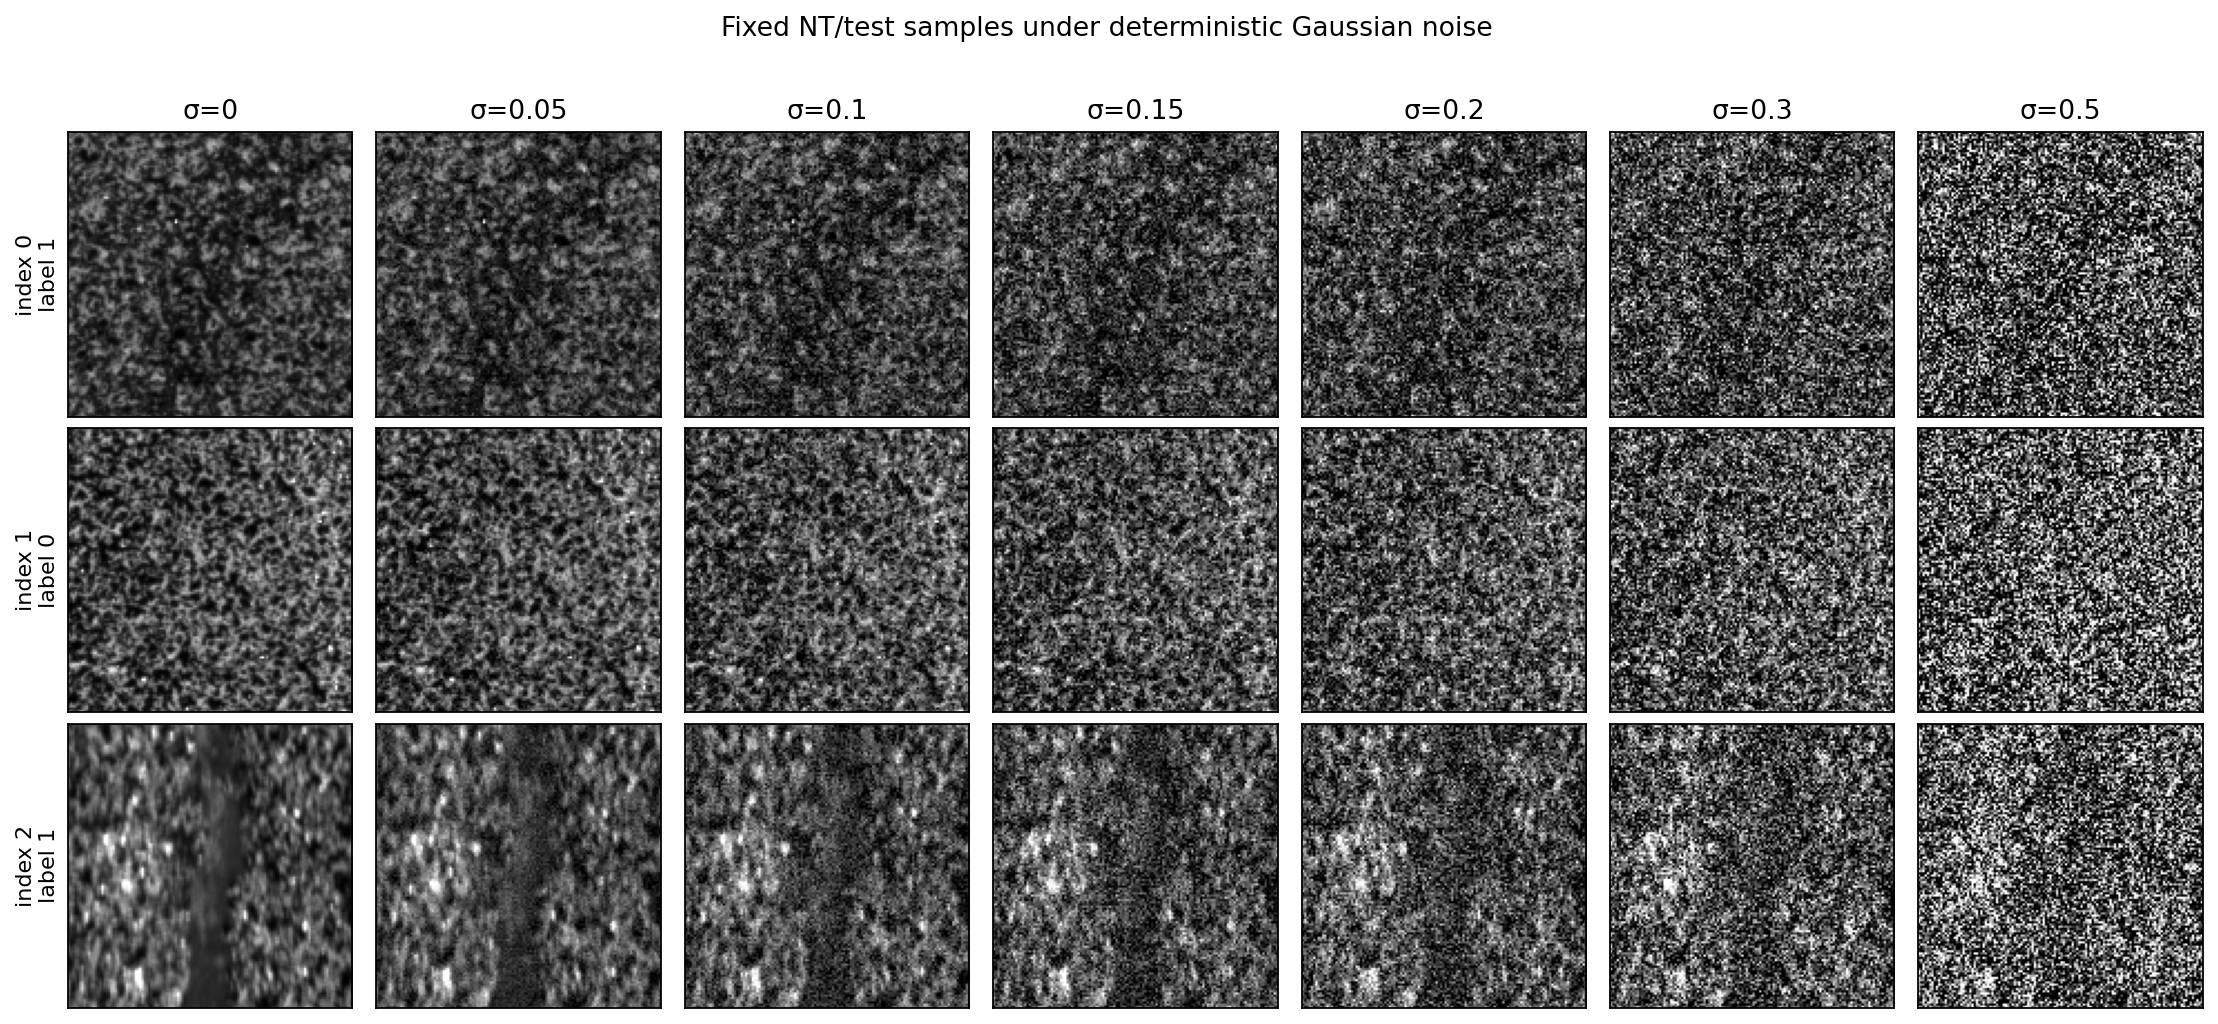
\includegraphics[width=0.84\linewidth]{tasks/task_2_robustness/results/noise_gallery.png}
\captionof{figure}{Fixed NT/test samples across all evaluated noise levels.}
\label{fig:t2-gallery}
\end{center}

\RunHead{Discussion}
Clean accuracy is \TaskTwoCleanAccuracy\%; it falls to 79.01\% at
$\sigma=0.05$ and 50.78\% at $\sigma=0.10$, the first objective failure. Therefore the model
does not fail at the light-noise setting $\sigma=0.05$ under the stated rule, but it fails at
$\sigma=0.10$ because both failure criteria are essentially met: the drop from clean accuracy
is far above 20 percentage points and the mean accuracy is near binary chance. For
$\sigma\geq0.15$, accuracy remains at approximately 50.35\%, so additional noise no longer
causes meaningful measured degradation because performance has already collapsed.
The gallery shows increasing speckle and loss of fine morphology. In the gallery, \(\sigma=0.05\) preserves main
specimen shape with visible grain, \(\sigma=0.1\) masks fine structure, and
\(\sigma=0.3,0.5\) are dominated by speckle.
\\ \\
The robustness characteristic is a threshold-like behavior: small corruption is tolerated only
partly, but once local grayscale texture is sufficiently distorted the classifier behaves close
to guessing. This suggests that the baseline relies more on fine local contrast and texture
cues than on coarse, noise-stable shape information.

\CodePath{tasks/task_2_robustness/}
\TaskEnd{2}

\TaskPage{3}{Activation Maps and Grad-CAM}

\RunHead{Approach}
Forward hooks capture activation maps after all three convolution/ReLU depths; Grad-CAM
targets each prediction at the final convolution. Four fixed NT/test indices cover correct
predictions from both classes and both error directions. Hooks and gradients are removed after
use. These methods diagnose representations; Grad-CAM is model-localized evidence, not causal
proof.
\\ \\
Both scripts reload the frozen Task 0 checkpoint, apply its preprocessing metadata, save
300-DPI figures, and write machine-readable metadata with sample indices, labels, confidence,
layer names, checkpoint hash, and hook/gradient cleanup checks.

\RunHead{Running the code}
The full workflow of this task is reproduced from the repository root with:
\begin{small}
	\begin{verbatim}
		conda run -n cnn_project python tasks/task_3_interpretability/activation_maps.py \
		--checkpoint tasks/task_0_baseline_cnn/results/best_model.pt \
		--indices 1 0 88 7 --device cpu \
		--output-dir tasks/task_3_interpretability/results/activation_maps
		conda run -n cnn_project python tasks/task_3_interpretability/gradcam.py \
		--checkpoint tasks/task_0_baseline_cnn/results/best_model.pt \
		--indices 1 0 88 7 --device cpu \
		--output-dir tasks/task_3_interpretability/results/gradcam
	\end{verbatim}
\end{small}

\RunHead{Results}
\begin{table}[h]
\centering
\small
\caption{Stable samples recorded in both interpretability metadata files.}
\label{tab:t3-samples}
\begin{tabular}{rllrr}
\toprule
Index & Role & True & Predicted & Confidence (\%) \\
\midrule
\TaskThreeRows
\bottomrule
\end{tabular}
\end{table}

\subsection*{Activation Maps}
\RunHead{Explanation and graph}
Activation maps show intermediate feature responses as the image passes through the CNN. The
figure reports the original image, true and predicted labels, confidence, class scores, the
channel-mean activation, and the strongest channels at each depth. Panels are independently
min-max scaled, so they are used to compare spatial patterns within a panel rather than absolute
activation magnitude across layers.

\begin{figure}[h]
\centering
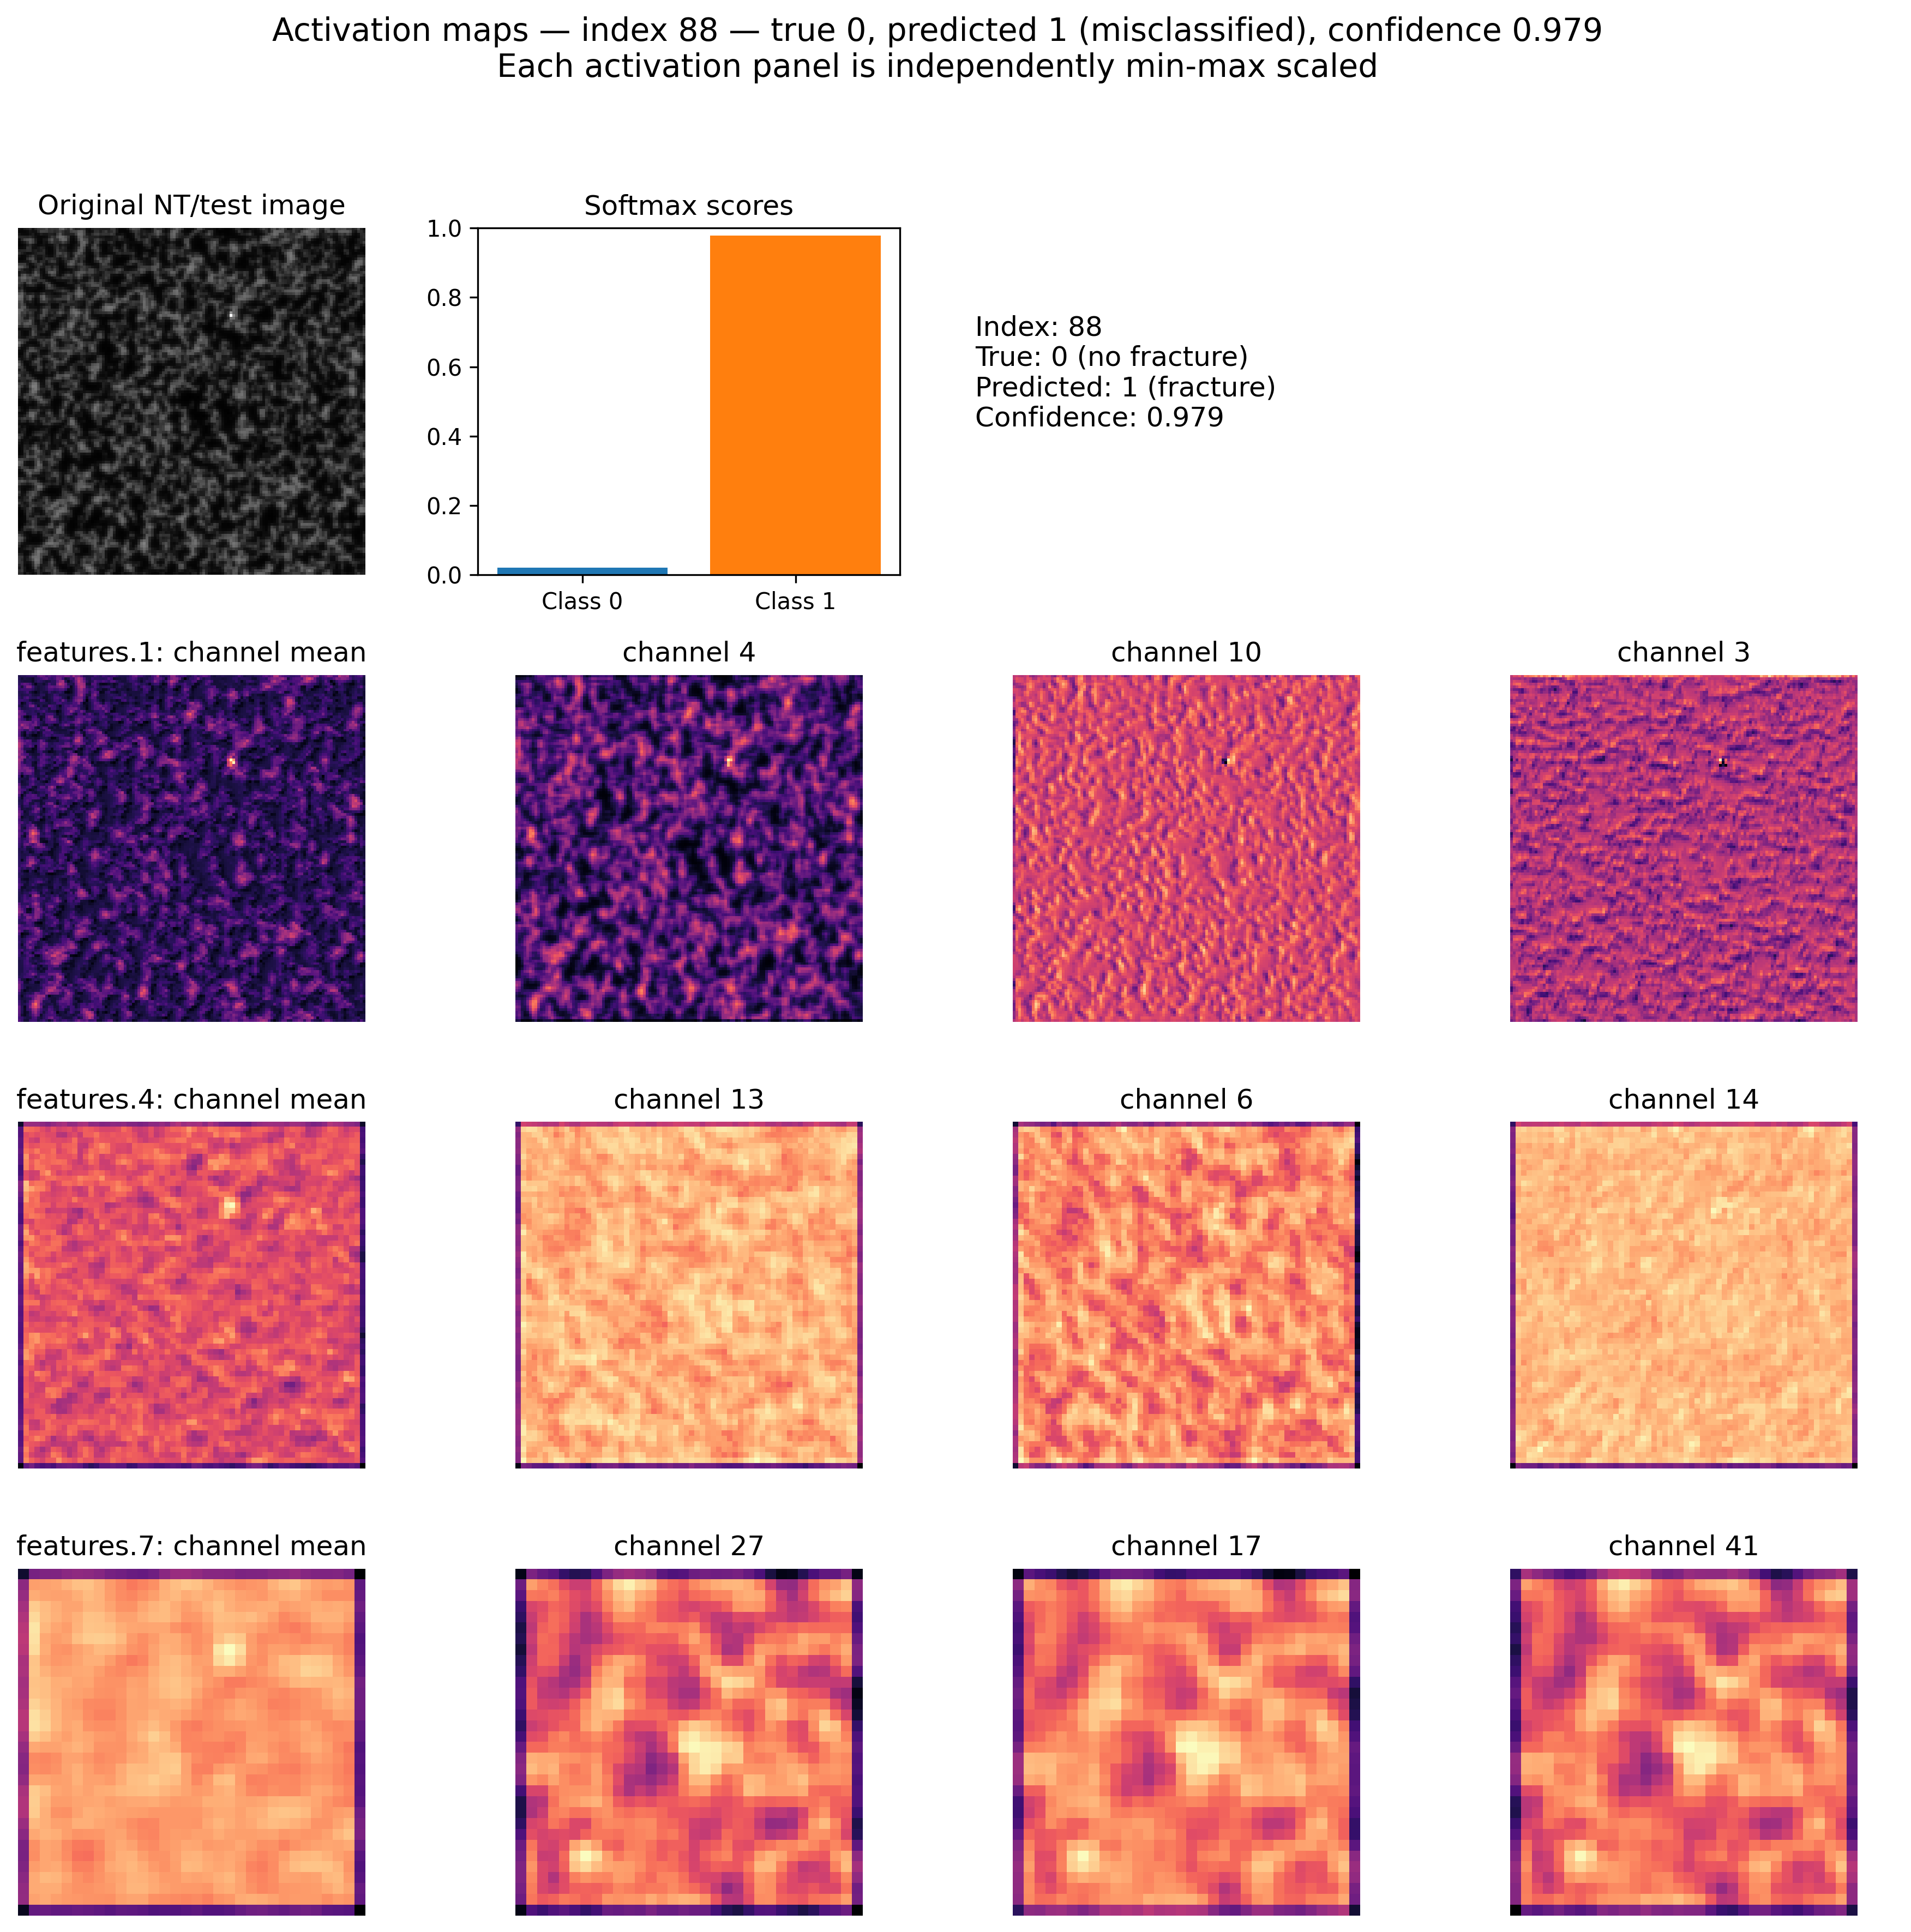
\includegraphics[width=0.50\linewidth]{tasks/task_3_interpretability/results/activation_maps/act_0088_fp.png}
\caption{Multi-depth activation hierarchy for false-positive sample \TaskThreeFalsePositiveIndex.}
\label{fig:t3-activation}
\end{figure}

\RunHead{Discussion}
The representation changes from local to abstract. At the first depth, feature maps retain
fine specimen texture, edges, and local contrast at nearly input resolution. At the middle
depth, these small responses are pooled into smoother regions, so individual pixels matter less
than local texture patches and larger contrast transitions. At the final depth, the maps are
coarse and spatially selective: only a few regions remain strongly active. This suggests that
the CNN has learned a hierarchy of visual correlations: early filters detect texture/edge
primitives, middle filters combine them into broader specimen structures, and late filters
highlight patches that the classifier can associate with class evidence. The inspected false
positive shows that similar late activations can support a confident but wrong class-1 decision,
so the features are informative but not perfectly aligned with a human fracture template.

\subsection*{Grad-CAM}
\RunHead{Explanation and graphs}
Grad-CAM is computed at the final convolutional layer \texttt{features.6} and targets the
model's predicted class for each sample. The heatmap therefore highlights image regions that
most support the model's own prediction, not necessarily the true label and not a causal proof.

\begin{figure}[h]
\centering
\begin{minipage}[c]{0.49\linewidth}
\centering
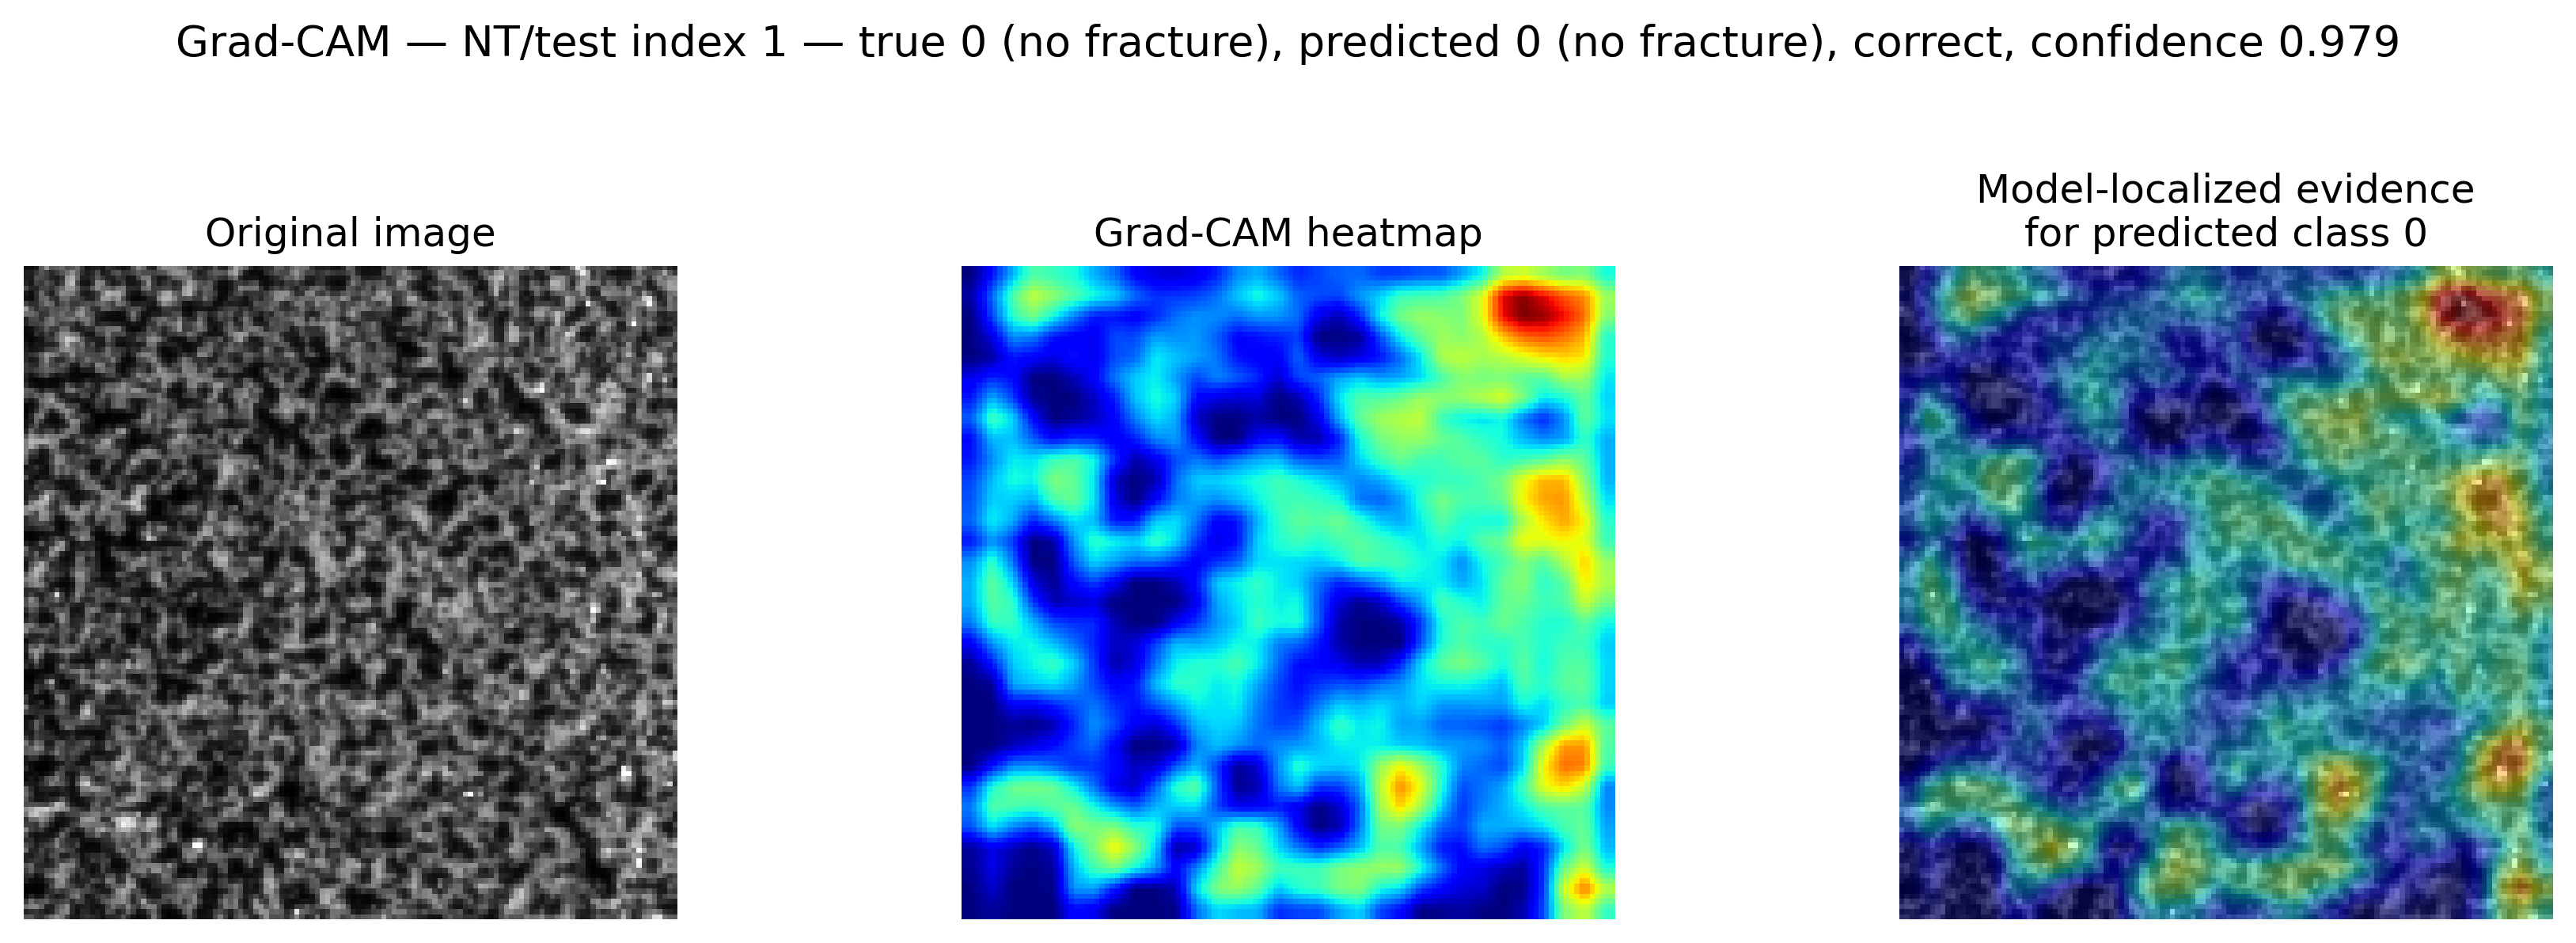
\includegraphics[width=\linewidth]{tasks/task_3_interpretability/results/gradcam/gradcam_index_0001_correct_class_0.png}
\small Correct class 0: distributed class-0 evidence.
\end{minipage}\hfill
\begin{minipage}[c]{0.49\linewidth}
\centering
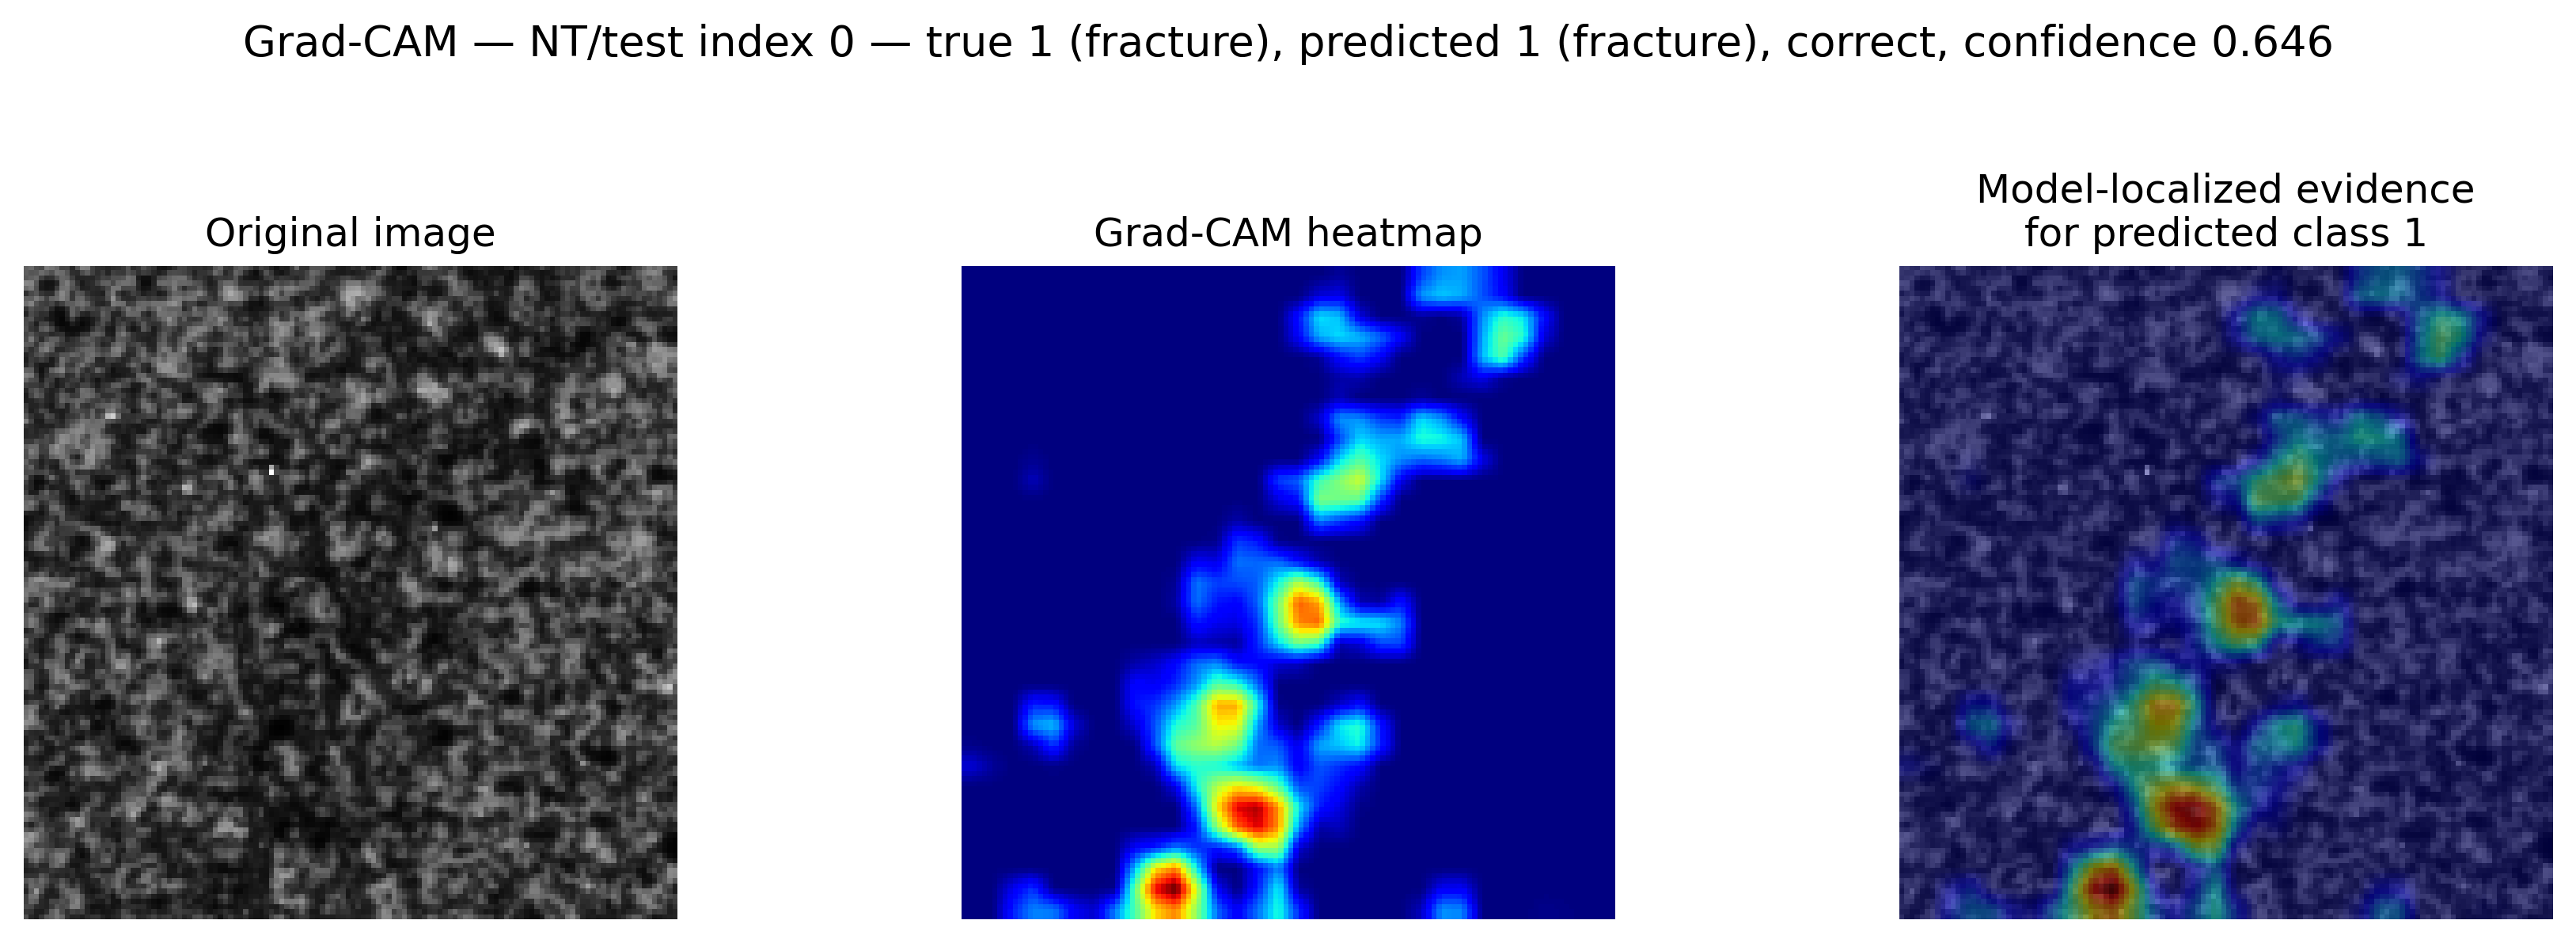
\includegraphics[width=\linewidth]{tasks/task_3_interpretability/results/gradcam/gradcam_index_0000_correct_class_1.png}
\small Correct class 1: compact fracture-class hotspots.
\end{minipage}

\vspace{2mm}
\begin{minipage}[c]{0.49\linewidth}
\centering
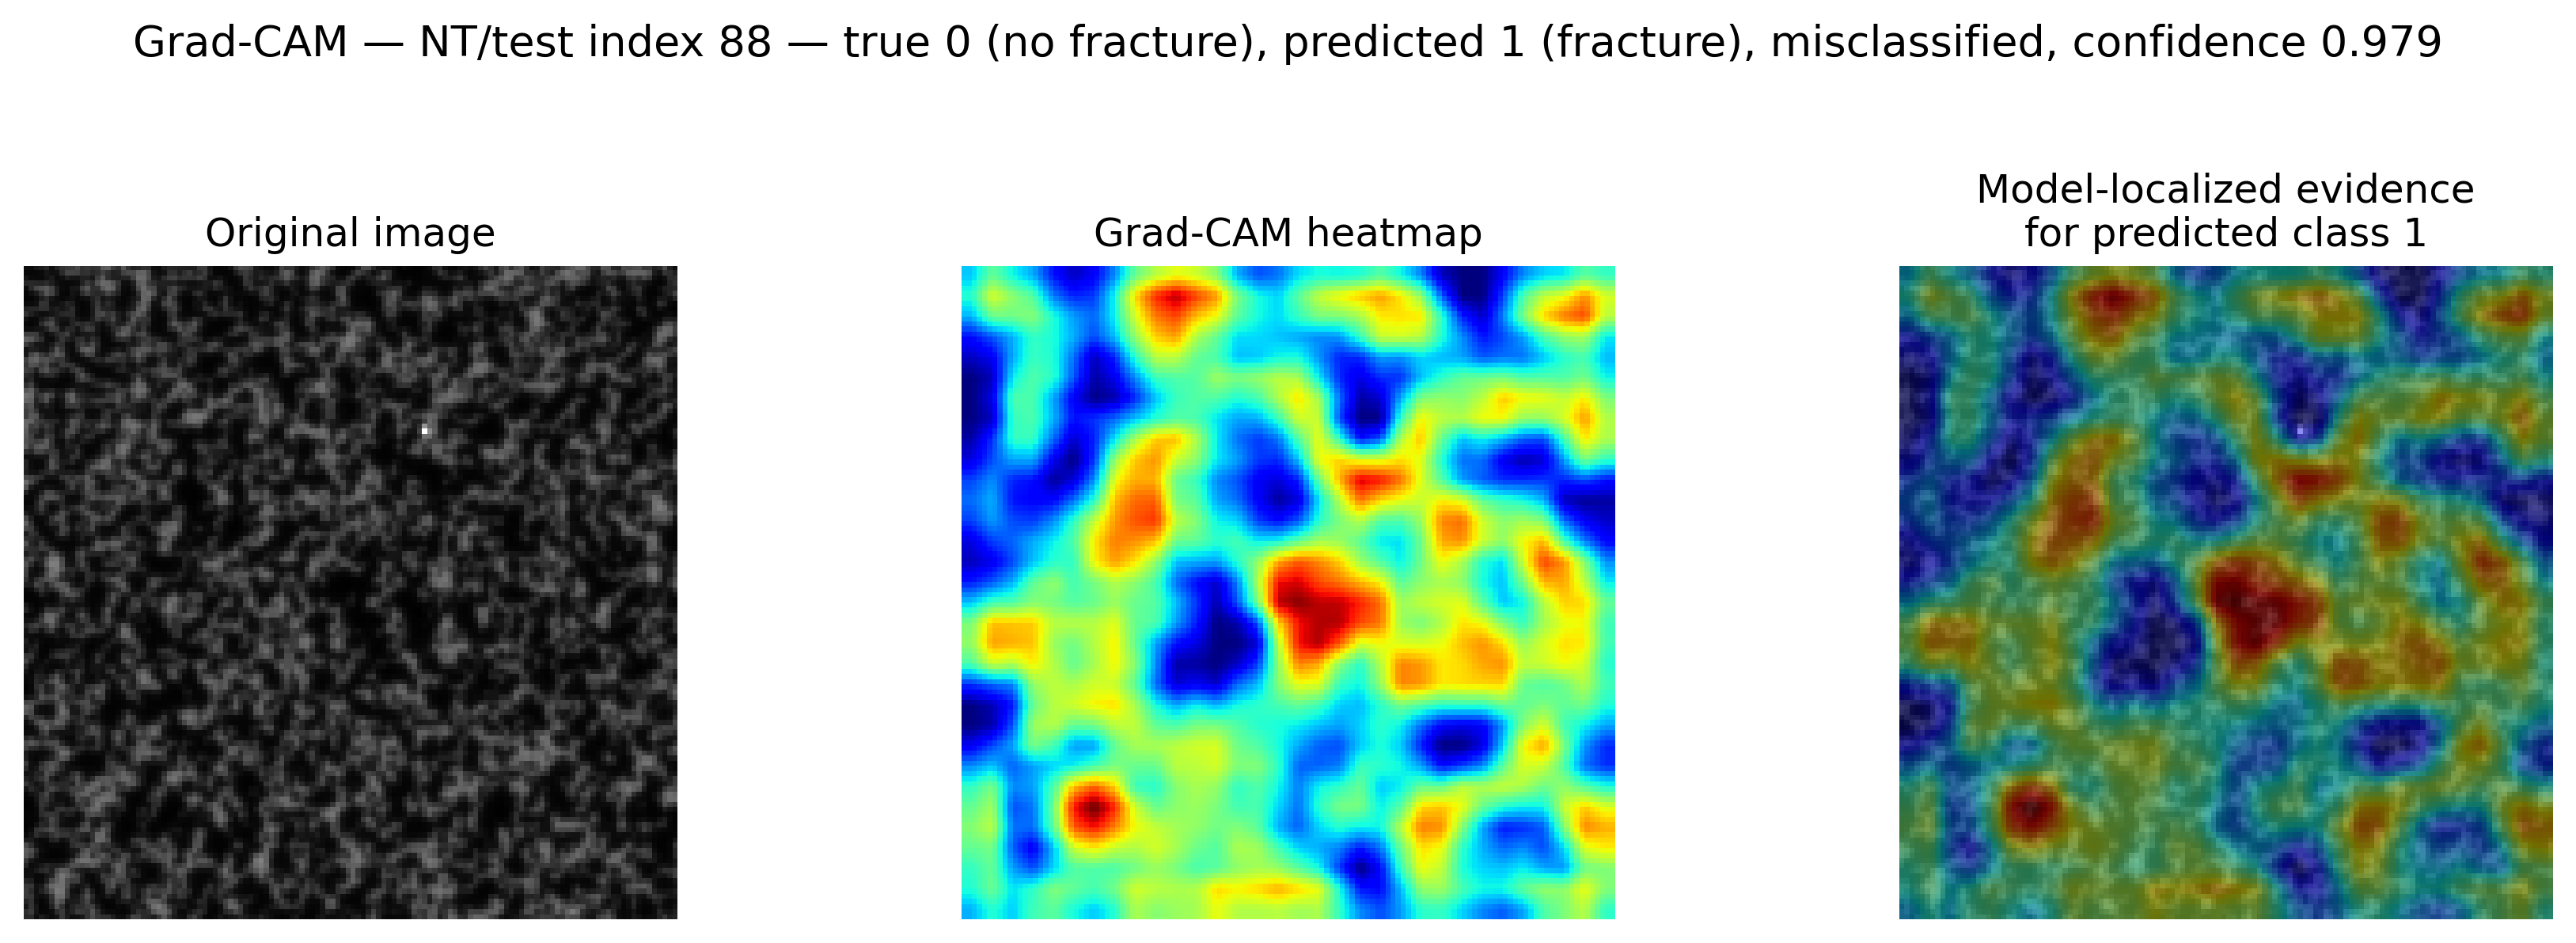
\includegraphics[width=\linewidth]{tasks/task_3_interpretability/results/gradcam/gradcam_index_0088_false_positive.png}
\small False positive: confident but misleading class-1 evidence.
\end{minipage}\hfill
\begin{minipage}[c]{0.49\linewidth}
\centering
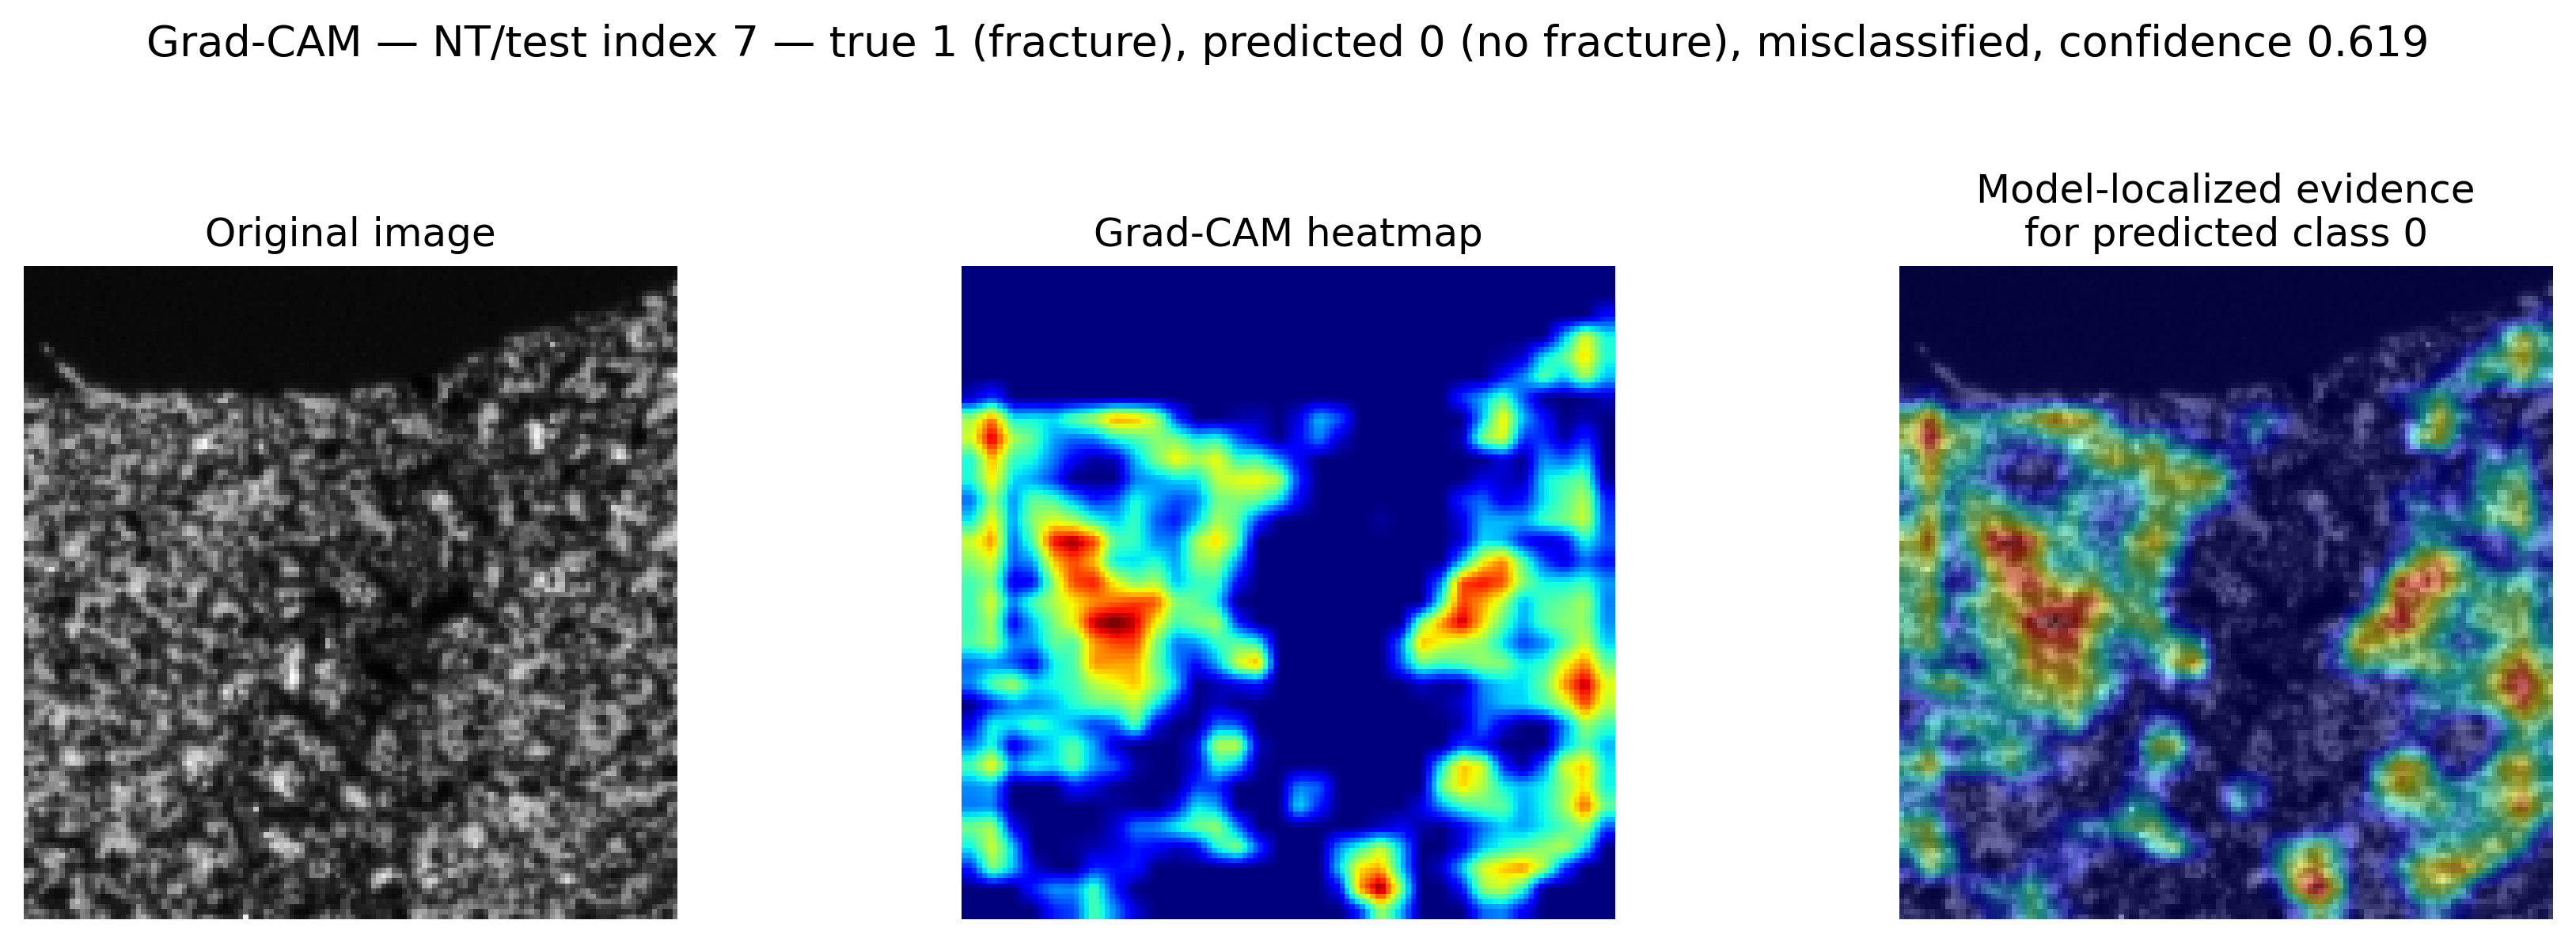
\includegraphics[width=\linewidth]{tasks/task_3_interpretability/results/gradcam/gradcam_index_0007_false_negative.png}
\small False negative: class-0 evidence on boundary/interior patches.
\end{minipage}
\caption{Predicted-class Grad-CAM evidence for correct and incorrect fixed samples.}
\label{fig:t3-interpretability}
\end{figure}

\RunHead{Discussion}
For the correct class-1 sample, influential regions are several compact hotspots along the
central/lower specimen area and near the upper-right region; the model does not attend uniformly
to the whole image. For the correct class-0 sample, class-0 evidence is more distributed, with
one strong upper-right hotspot and weaker peripheral regions. The false positive is important:
the model predicts fracture with \TaskThreeFalsePositiveConfidence\% confidence, but its
evidence is diffuse across textured regions rather than one uniquely convincing structure, so
attention can look plausible while supporting an error. For the false negative, the class-0
prediction is supported by specimen boundary and interior patches while much of the central dark
region receives little weight.

\RunHead{What the CNN has learned}
Across both visualization methods, the CNN appears to have learned local grayscale texture
density, contrast transitions, specimen boundaries, and coarse localized patches. It has not
learned an explicitly human-readable rule such as ``find one fracture line.'' The features are
partially interpretable: early and middle layers visibly track texture and boundaries, while
Grad-CAM gives coarse localization of final evidence. However, similar hotspots occur in correct
and incorrect cases, and the final heatmaps have only coarse spatial resolution, so the
visualizations should be read as diagnostics of this model's evidence rather than complete
explanations of the physical defect.

\CodePath{tasks/task_3_interpretability/}
\TaskEnd{3}

\TaskPage{4}{Confusion-Matrix Error Analysis}

\RunHead{Approach}
The frozen Task 0 model is evaluated once on all \TaskZeroTestSize{} NT/test samples in index
order. Predictions, confidence, correctness, raw/row-normalized matrices, class metrics, and
stable false-positive/false-negative gallery indices are saved. Precision, recall, and F1 are
reported because accuracy alone hides directional errors.
Here, precision means ``of the images predicted as a class, how many are correct''; recall means
``of the true images of a class, how many are found''; F1 is the harmonic mean of precision and
recall; support is the number of true test samples in that class.


\RunHead{Running the code}
The full workflow of this task is reproduced from the repository root with:
\begin{small}
	\begin{verbatim}
		conda run -n cnn_project python tasks/task_4_confusion_matrix/analysis.py \
		--checkpoint tasks/task_0_baseline_cnn/results/best_model.pt \
		--reference-metrics tasks/task_0_baseline_cnn/results/metrics.json \
		--device cpu --batch-size 64 --workers 0 --max-per-error 6 \
		--output-dir tasks/task_4_confusion_matrix/results
	\end{verbatim}
\end{small}

\RunHead{Results}
\begin{table}[h]
\centering
\small
\caption{Per-class test metrics; overall accuracy is \TaskFourAccuracy\% and macro F1 is \TaskFourMacroFOne\%.}
\label{tab:t4-metrics}
\begin{tabular}{lrrrr}
\toprule
Class & Precision (\%) & Recall (\%) & F1 (\%) & Support \\
\midrule
0 & \TaskFourClassZeroPrecision & \TaskFourClassZeroRecall & \TaskFourClassZeroFOne & \TaskFourClassZeroSupport \\
1 & \TaskFourClassOnePrecision & \TaskFourClassOneRecall & \TaskFourClassOneFOne & \TaskFourClassOneSupport \\
\bottomrule
\end{tabular}
\end{table}

\vspace{1cm}

\begin{figure}[h]
\centering
\begin{minipage}[c]{0.3\linewidth}
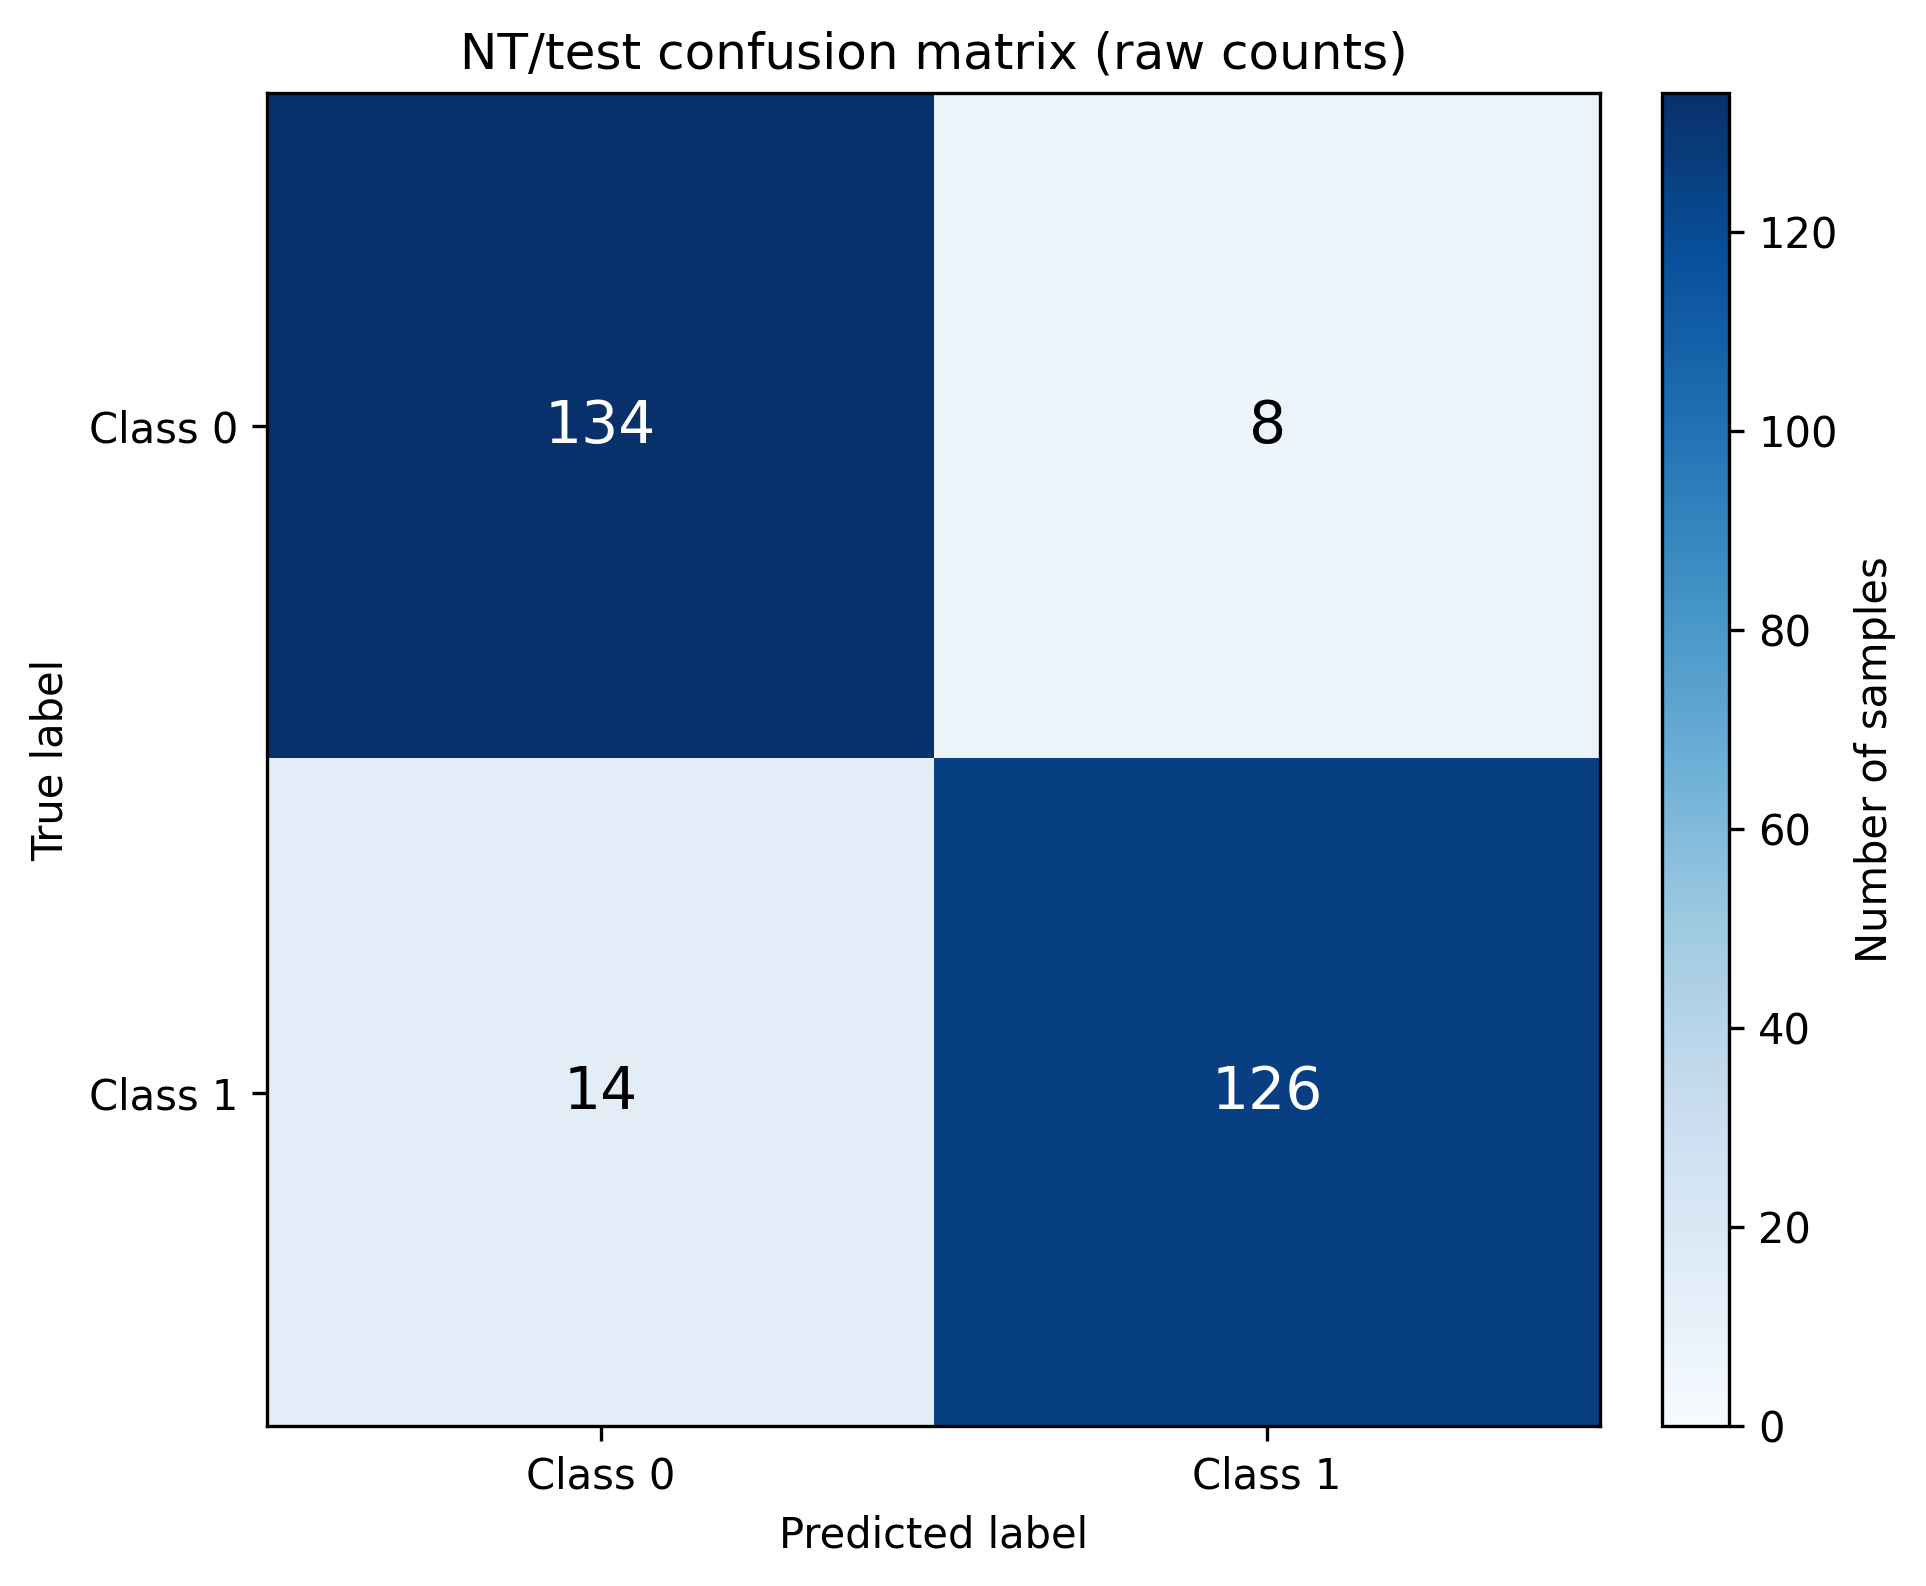
\includegraphics[width=\linewidth]{tasks/task_4_confusion_matrix/results/confusion_matrix_counts.png}
\small Raw counts.
\end{minipage}
\begin{minipage}[c]{0.3\linewidth}
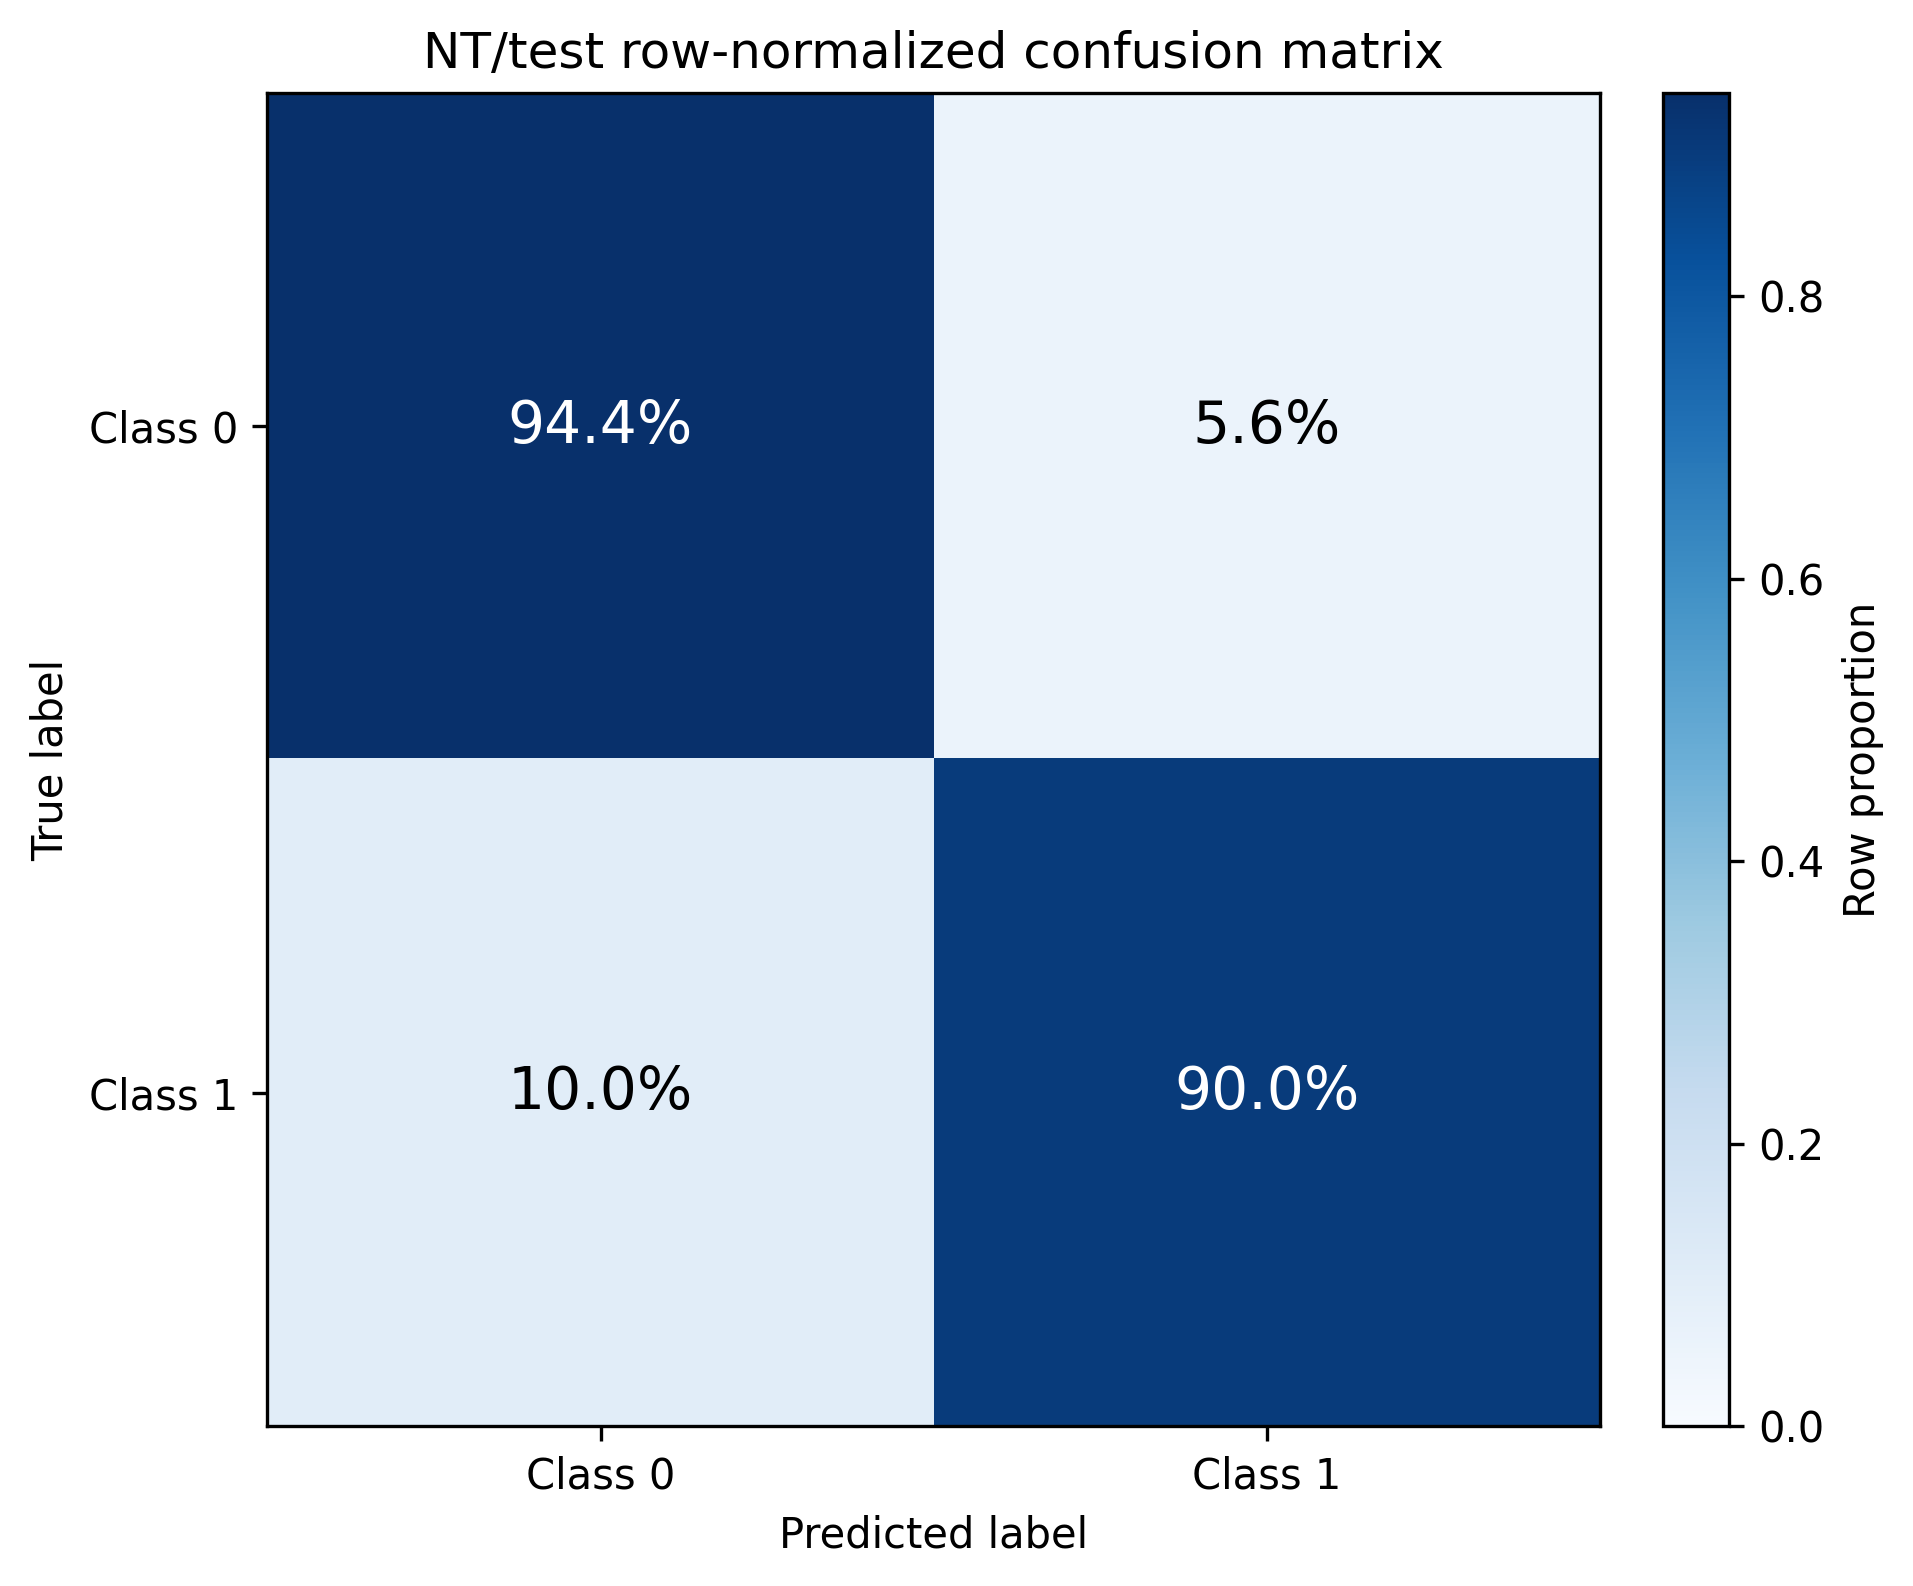
\includegraphics[width=\linewidth]{tasks/task_4_confusion_matrix/results/confusion_matrix_normalized.png}
\small Row-normalized.
\end{minipage}\vspace{0.5cm}
\begin{minipage}[c]{0.75\linewidth}
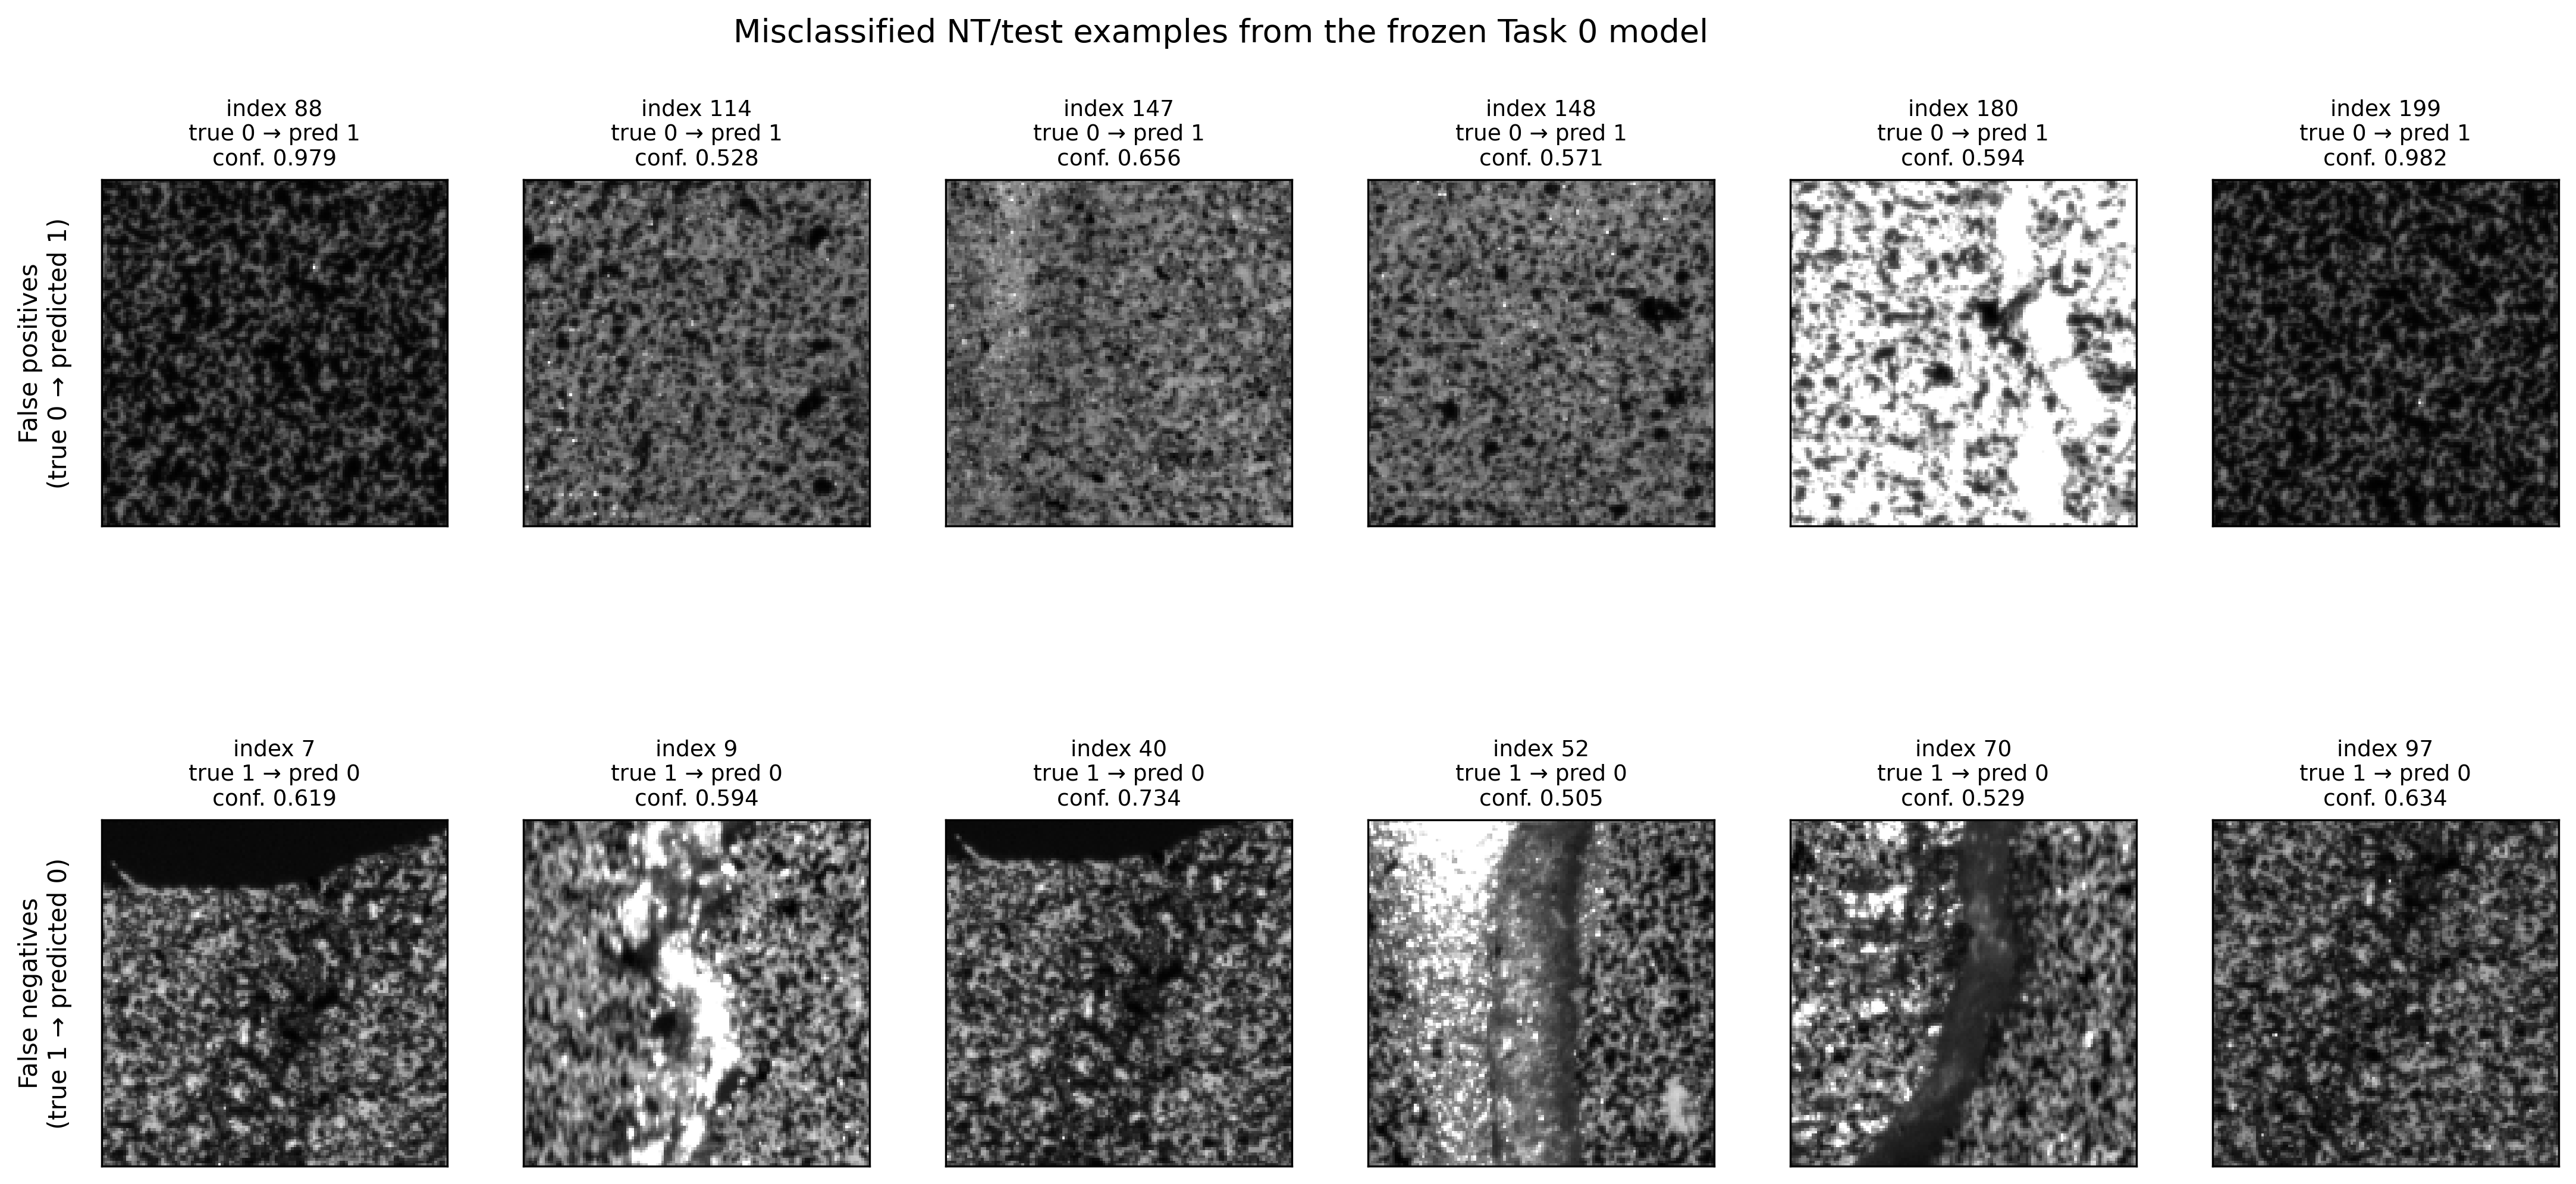
\includegraphics[width=\linewidth]{tasks/task_4_confusion_matrix/results/misclassified_gallery.png}
\small Misclassified gallery.
\end{minipage}
\caption{Raw-count and row-normalized confusion matrices plus inspected false positives/negatives.}
\label{fig:t4-errors}
\end{figure}

\RunHead{Discussion}
Class 1 is harder to recover: its recall is
\TaskFourClassOneRecall\% versus \TaskFourClassZeroRecall\% for class 0, producing
\TaskFourFalseNegatives{} false negatives and \TaskFourFalsePositives{} false positives.
Its precision is higher (\TaskFourClassOnePrecision\%), so when the model predicts class 1 it
is usually right; the main weakness is missing true class-1 samples. This suggests that some
fracture-like cases are not represented strongly enough by the learned class-1 evidence.

\textbf{What do misclassified images have in common?} The inspected false positives do not
share one clear global brightness pattern: they span dark, mid-tone, and bright images. Several
selected false negatives contain strong central bands, high-contrast structures, or specimen
boundaries, although this is not universal. A cautious interpretation is that illumination
changes and boundary/texture artifacts can interfere with the local cues used by the baseline
CNN; the gallery is evidence for a pattern, not causal proof.

\textbf{How to improve failure cases?} Improvements should be selected on NT/val, not by tuning
to these test errors. Useful follow-up experiments are: add train-only brightness/contrast and
small spatial augmentations to reduce sensitivity to illumination and boundary placement; tune a
class-1 decision threshold on validation data if missing fractures is more costly than false
alarms; use validation-set hard-example mining so difficult class-1-like cases receive more
training weight; test a justified crop or segmentation step that removes irrelevant borders
without removing fracture information; and collect or label more samples resembling the
high-contrast/boundary cases. \textbf{Limitation:} the gallery shows 12 of 22 errors from one
checkpoint, softmax confidence is uncalibrated, and the proposed remedies require new
validation-controlled experiments before another test evaluation.

\CodePath{tasks/task_4_confusion_matrix/}
\TaskEnd{4}

\TaskPage{5}{NT/UT Cross-Dataset Generalization}

\RunHead{Approach}
Identical Task 0 architectures and protocols train separately on NT and UT, with seed 42 reset
for each. Each checkpoint is selected only by its source validation loss (epochs
\TaskFiveNTBestEpoch{} and \TaskFiveUTBestEpoch{}) and locked before either test split is opened.
Identity preprocessing from each source checkpoint is applied unchanged to both targets.
The PDF lists only NT$\rightarrow$UT and UT$\rightarrow$NT yet retains contradictory ``3$\times$3''
wording; the PDF's ASB warning makes the valid matrix 2$\times$2.

\RunHead{Running the code}
The full experiment is run from the repository root with:
\begin{small}
\begin{verbatim}
conda run -n cnn_project python tasks/task_5_cross_dataset/cross_evaluation.py \
  --seed 42 --epochs 30 --batch-size 64 --learning-rate 0.001 \
  --device cpu --workers 0 --early-stopping-patience 6 \
  --output-dir tasks/task_5_cross_dataset/results
\end{verbatim}
\end{small}
The script first trains and locks both source checkpoints, then opens NT/test and UT/test for
the four frozen evaluations. A separate \texttt{--train-only} mode exists for checking training
without opening any test split.

\RunHead{Results}

\begin{center}
	
\begin{minipage}[t]{0.43\linewidth}
\centering
\captionof{table}{Accuracy matrix (\%); rows are source and columns are target test domains.}
\label{tab:t5-matrix}
\small
\begin{tabular}{lrr}
\toprule
Source & NT & UT \\
\midrule
NT & \TaskFiveNTNT & \TaskFiveNTUT \\
UT & \TaskFiveUTNT & \TaskFiveUTUT \\
\bottomrule
\end{tabular}

\vspace{4mm}
\begin{tabular}{lrr}
\toprule
Source & Selected epoch & CPU time (s) \\
\midrule
NT & \TaskFiveNTBestEpoch & \TaskFiveNTTrainingSeconds \\
UT & \TaskFiveUTBestEpoch & \TaskFiveUTTrainingSeconds \\
\bottomrule
\end{tabular}
\end{minipage}

\vspace{1cm}

\begin{minipage}[t]{0.54\linewidth}
\centering
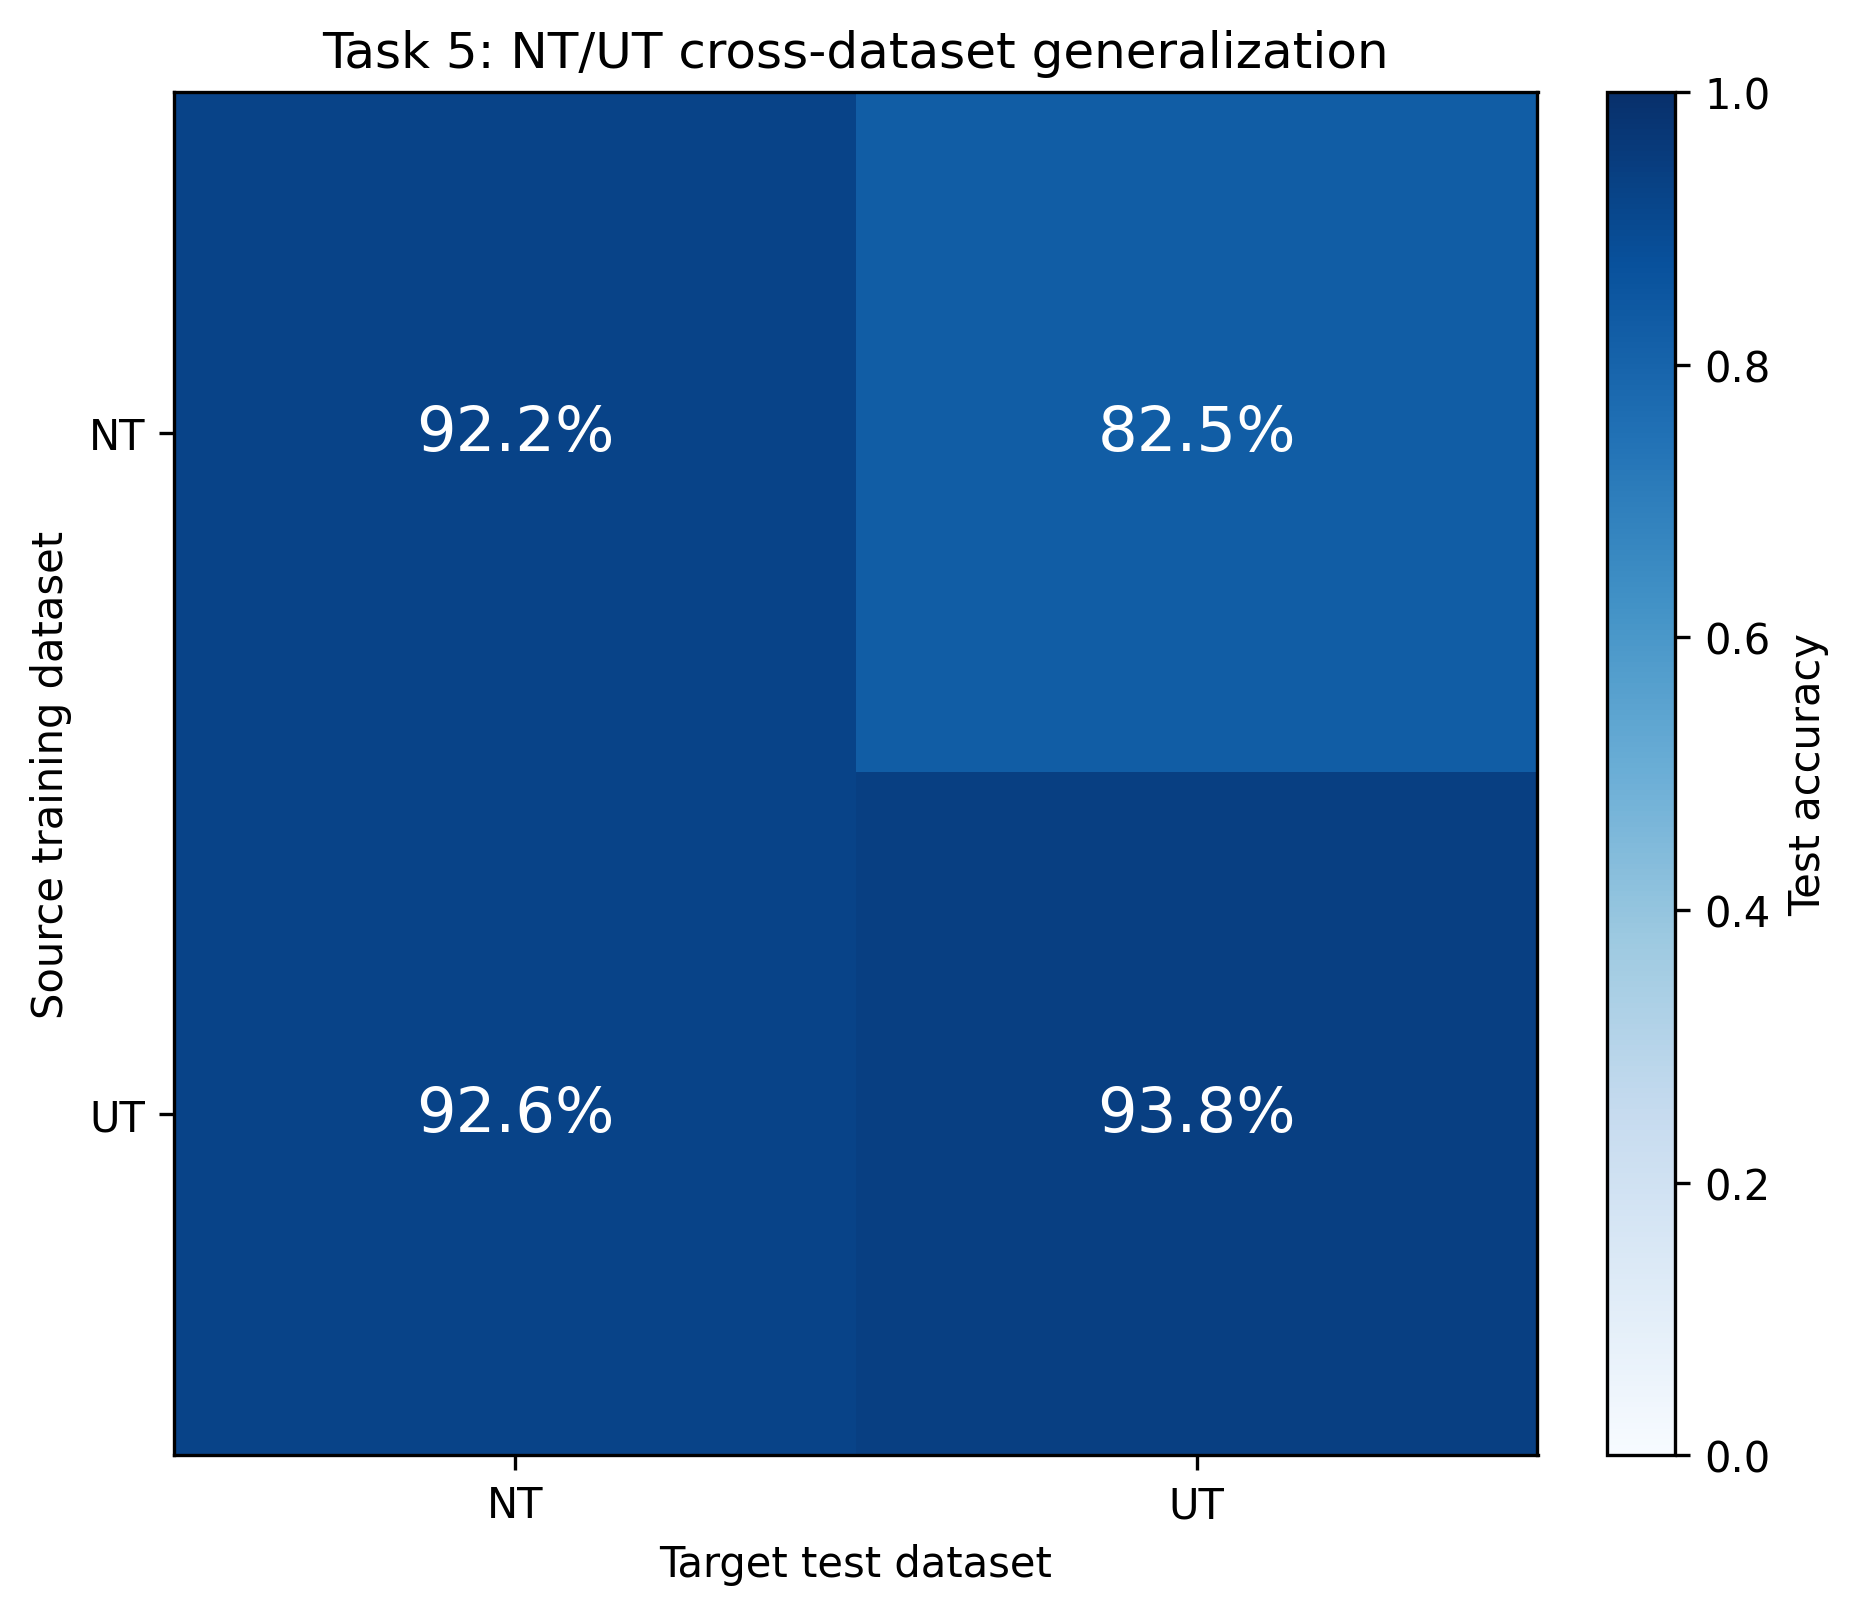
\includegraphics[width=0.82\linewidth]{tasks/task_5_cross_dataset/results/accuracy_heatmap.png}
\captionof{figure}{Within-domain diagonal and required cross-domain transfer.}
\label{fig:t5-heatmap}
\end{minipage}
\end{center}

\RunHead{Discussion}
Transfer is asymmetric. NT$\rightarrow$UT reaches
\TaskFiveNTUT\%, which is \TaskFiveNTUTSourceDrop{} points below NT$\rightarrow$NT and
\TaskFiveNTUTTargetGap{} points below the UT-trained model on UT. Its confusion matrix has
\TaskFiveNTUTClassZeroErrors{} class-0 errors and \TaskFiveNTUTClassOneErrors{} class-1 errors,
so the drop is not a simple collapse to one predicted class; both UT classes are harder for the
NT-trained model. In contrast, UT$\rightarrow$NT reaches \TaskFiveUTNT\%, essentially matching
NT$\rightarrow$NT and differing by only one additional correct image. Therefore, the required
cross-domain result that clearly suffers is NT$\rightarrow$UT.
\\ \\
The NT model performs well on its own domain but
loses accuracy when only the target domain changes to UT, which is direct evidence of domain
shift. Because preprocessing is identical and source-derived, the shift is not caused by
target-specific normalization. The stronger UT$\rightarrow$NT result suggests that UT-trained
features overlap well with NT features: the UT model learns texture, edge, and contrast cues
that still work on NT. The weaker NT$\rightarrow$UT result suggests that NT does not cover some
UT variability, possibly in texture statistics, contrast, illumination, or specimen appearance.
This is a feature-similarity statement from transfer behavior, not a claim about the physical
cause of the shift.
\\ \\
If deployment target images resemble UT, training only on NT is risky.
A practical improvement would be to train on source data that better spans both domains, use
validation-controlled augmentation for intensity/contrast variation, or develop domain
adaptation/normalization choices using training and validation data only. \textbf{Limitation:}
one seed, unequal test sizes, identity preprocessing, and no domain adaptation prevent broader
claims. The saved leakage audit verifies no target tuning.

\CodePath{tasks/task_5_cross_dataset/}
\TaskEnd{5}

\clearpage

\section*{Conclusion}
This project built a reproducible CNN pipeline for the valid NT/UT fracture-image datasets
while excluding ASB because the assignment PDF warns that its labels are systematically wrong.
The Task 0 baseline already achieved \TaskZeroAccuracy\% on NT/test, showing that a compact
three-stage CNN can learn useful local texture and edge cues from the supplied microscopy
images. Hyperparameter optimization improved the locked NT/test result to \TaskOneTestAccuracy\%,
mainly by finding better training dynamics through learning rate, batch size, AdamW, and a
moderate dropout setting. However, the robustness experiment showed that high clean accuracy
does not imply stability: performance dropped sharply under Gaussian noise and first failed at
$\sigma=\TaskTwoFirstFailure$, indicating strong dependence on fine grayscale texture.

The interpretability and error-analysis tasks make the model behavior more concrete. Activation
maps evolve from fine edges and texture to coarse localized evidence, and Grad-CAM shows that
predictions are driven by localized patches rather than a single human-readable fracture rule.
The confusion matrix confirms that class 1 is harder to recover by recall, with
\TaskFourFalseNegatives{} false negatives versus \TaskFourFalsePositives{} false positives.
Inspected mistakes suggest that high-contrast bands, boundaries, and illumination variation can
interfere with the learned cues, although these observations are diagnostic rather than causal.
Cross-dataset evaluation revealed asymmetric transfer: UT-trained features generalize well to NT
(\TaskFiveUTNT\%), but NT-trained features lose accuracy on UT (\TaskFiveNTUT\%), so deployment
should account for domain shift and source/target similarity.

The main lesson is that a CNN result should not be judged by a single clean test accuracy. A
defensible workflow needs strict split separation, validation-only model selection, locked
checkpoint metadata, robustness checks, interpretability diagnostics, error inspection, and
cross-domain testing.

\clearpage

\end{document}
